\documentclass[12pt,a4paper,titlepage,oneside]{article}

% --- Paquets de base ---
\usepackage[utf8]{inputenc}
\usepackage[T1]{fontenc}
\usepackage[french]{babel}
\usepackage[top=1.5cm, bottom=5cm]{geometry}
\usepackage{graphicx}
\usepackage{listings}
\usepackage{array, pdfpages}
\usepackage[breaklinks]{hyperref}
\usepackage{tabularx}
\usepackage{makecell}
\usepackage{float}
\usepackage[export]{adjustbox}
% --- Bibliographie ---
\usepackage[
style=numeric,
sorting=ynt
]{biblatex}

\addbibresource{biblio.bib}

% --- Mise en page (Header/Footer) ---
\usepackage{fancyhdr}
\pagestyle{fancy}
\fancyhf{} 
\rhead{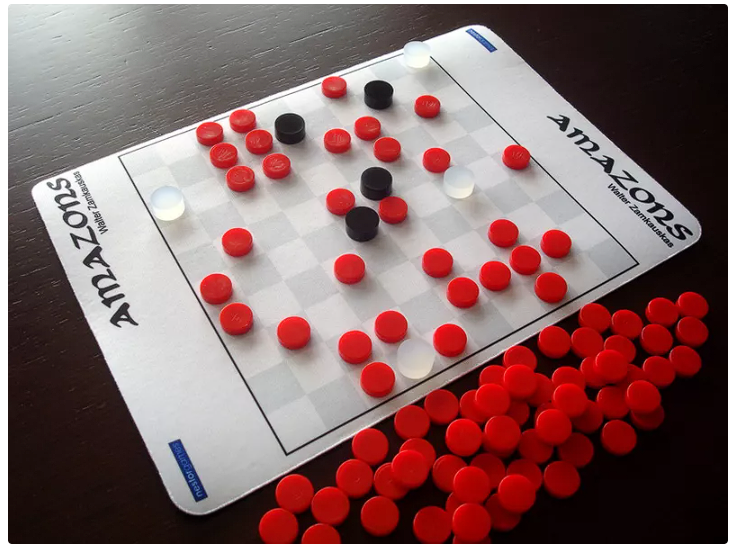
\includegraphics[width=2cm]{Amazones}} 
\cfoot{\thepage} 
\headheight = 2cm
\headsep = 1.5cm

% --- Personnalisation des titres ---
\usepackage{titlesec}
\titleformat{\part}[display]
  {\normalfont\huge\bfseries}
  {}
  {0pt}
  {\huge}

\counterwithin{section}{part}
\renewcommand{\thepart}{\arabic{part}}
\begin{document}

    % --- Page de garde ---
    \begin{titlepage}
        \fontfamily{pag}\selectfont
        \begin{center}\normalsize
            \MakeUppercase{Informatique M1 \hfill Groupe Amazone C \hfill 2025-2026}
        \end{center}
        \vspace*{0.1cm}
        \hrule
        \vspace*{0.2cm}
        \vspace*{2cm}
        \begin{center}\Huge
            \textsc{\textbf{Rapport Projet M1}}
        \end{center}
        \hrule
        \begin{center}
            \MakeUppercase{Rapport effectué dans le cadre du projet de semestre 8}
        \end{center}
        \vspace*{2cm}
        \begin{center}\Large
            Nicolas \textsc{Caminade}\\ \vspace{0.3cm}
            Tanguy \textsc{Decabrat}\\ \vspace{0.3cm}
            Anya \textsc{Bazizi}\\ \vspace{0.3cm}
            Younes \textsc{Ouaammou}\\ \vspace{0.3cm}
            Thomas-Alexandre \textsc{Moreau}
        \end{center}
        \vfill
        \begin{center}\normalsize
            \MakeUppercase{Rapport Projet --- Semestre 8}
        \end{center}
    \end{titlepage}

    % --- Sommaire ---
    \newpage
    \renewcommand{\contentsname}{Sommaire}
    \setcounter{tocdepth}{1} 
    \tableofcontents
    \newpage

    % --- Corps du document ---
    \markboth{}{} 
    \normalsize

    \setcounter{part}{0}

    \part{Présentation du projet}
\section{Historique des Amazones}

Le Jeu des Amazones, créé par l'argentin Walter Zamkauskas en 1988, est un jeu de stratégie se jouant à deux joueurs. Il se joue sur un plateau carré sur lequel sont placées des pièces s'appelant des "amazones". Chaque joueur contrôle un nombre prédéterminé d'amazones selon la taille du plateau, en général 4. L'objectif est simple : restreindre les mouvements de l'adversaire tout en maximisant ses propres possibilités de déplacement.

\medskip

Ce jeu contient une énorme quantité de combinaison possible et il est souvent comparé au Go ou aux Échecs en raison de son absence de hasard et de son système d'information complète, où les deux adversaires s'affrontent avec des pièces identiques. Sa particularité réside dans sa mécanique de jeu : chaque coup consiste en un déplacement suivi d'un tir de flèche qui bloque définitivement une case du plateau.

\medskip

Cette dynamique génère une croissance exponentielle du nombre de positions possibles au fur et à mesure que la partie progresse. La difficulté computationnelle qui en découle est démontrée par la théorie de la complexité : 
\begin{itemize}
    \item Déterminer qui va gagner une partie précise est un problème classé comme NP-difficile.
    \item Déterminer qui va gagner une partie de façon générale est classé comme PSPACE-complet.
\end{itemize}





    \section{Règles}

    Le Jeu des Amazones se pratique sur un damier, traditionnellement de $10 \times 10$ cases. Chaque joueur possède quatre amazones, placées dans une configuration initiale spécifique qui définit le point de départ .
    
    \paragraph{Objectif du jeu}Le but est de complètement bloquer les mouvement de l'adversaire en occupant ou en bloquant stratégiquement l'espace. La victoire est acquise lorsqu'un joueur parvient à bloquer toutes les amazones adverses, ne lui laissant plus aucune possibilité de mouvement.

    \newpage
     
    \paragraph{Déroulement d'un tour}Chaque action d'un joueur est impérativement composée de deux phases successives :
    \begin{enumerate}
    
    \item \textbf{Le déplacement :} Le joueur choisit l'une de ses amazones et la déplace en ligne droite (verticalement, horizontalement ou en diagonale) vers une case libre. Le mouvement est identique à celui de la dame aux échecs, mais l'amazone ne peut ni traverser ni s'arrêter sur une case occupée par une autre pièce ou une flèche.
    \item \textbf{Le tir de flèche :} Après son déplacement, cette même amazone doit tirer une flèche depuis sa nouvelle position. La flèche suit les mêmes règles de trajectoire qu'une amazone. La case d'arrivée de la flèche est alors marquée d'un blocage définitif pour le reste de la partie.
    \end{enumerate}
    \paragraph{Fin de partie et variantes}Contrairement à d'autres jeux de plateau, le Jeu des Amazones ne connaît pas de situation de match nul par répétition ou par épuisement de matériel. Puisque chaque tour réduit irrémédiablement le nombre de cases disponibles, le jeu se termine forcément par le blocage complet d'un joueur. Bien que le format $10 \times 10$ soit le standard, il existe des variantes sur des plateaux plus réduits ($6 \times 6$ ou $8 \times 8$) avec un nombre d'amazones adapté, permettant des parties plus rapides tout en conservant la complexité tactique du jeu.
    \\
    \begin{figure}[ht]
    \centering
    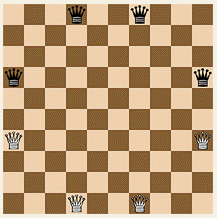
\includegraphics[width=0.30\textwidth]{defaultStateboard.png} 
    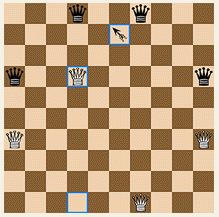
\includegraphics[width=0.30\textwidth]{1wallplacedboard.png}
    \caption{Évolution d'une partie : position initiale et premier coup \cite{img0} \cite{img1}}
\end{figure}

   

    
    \section{Complexité} \label{sec:complexite}
        Les Amazones est un jeu ayant une très grande complexité de départ \cite{Complexite}. La richesse des positions de jeu est telle qu'une exploration exhaustive de l'arbre des possibles est à proscrire, dû à l'explosion combinatoire des possibilités de jeu. De ce fait, utiliser la famille d'algorithmes comme Minimax ou Alpha-Beta, explorant l'arbre des possibles, avec un élagage classique où l'on doit atteindre des feuilles afin d'élaguer, n'est pas suffisant.
        
        Pour contourner cette explosion combinatoire, les approches modernes s'appuient sur la sélectivité : soit par des solveurs de preuve comme \textit{df-pn} (Song \& Müller), soit par des algorithmes de jeu utilisant du \textit{Forward Pruning} (élagage prospectif) ou des méthodes statistiques comme MCTS, afin de focaliser la recherche sur les chemins les plus intéréssants, en triant les coups possibles par un algorithme d'évaluation comme \textit{Upper Confidence bounds applied to Trees} (UCT), ou encore via du \textit{Machine Learning} intégré.
        
        Mais quelle est sa complexité par rapport à d'autres jeux ?
        

\begin{table}[h!]
    \centering
\renewcommand{\arraystretch}{1.5}
\resizebox{\textwidth}{!}{
\begin{tabular}{ | p{4.5cm} || c | c | c | }
    \hline
    % --- Première Ligne (En-têtes) ---
    \textbf{} & \textbf{Échecs} & \textbf{Amazones} & \textbf{Go} \\
    \hline

    % --- Reste du tableau ---
    Facteur Branch. Initial
    & $\mathtt{\sim}$ 20
    & \makecell{$\mathtt{\sim}$ 2176}
    & $\mathtt{\sim}$ 361 \\
    \hline
    Facteur Branch. Moyen
    & $\mathtt{\sim}$ 35
    & \makecell{$\mathtt{\sim}$ 374 joueur de départ \\ $\mathtt{\sim}$ 299 deuxième joueur}
    & $\mathtt{\sim}$ 250 \\
    \hline
    Nombre de tours moyen
    & $\mathtt{\sim}$ 80 
    & $\mathtt{\sim}$ 84 
    & $\mathtt{\sim}$ 150 \\
    \hline
    Cmplx. Arbre de jeu 
    & $\mathtt{\sim} 10^{123}$ 
    & $\mathtt{\sim}$ 1.09 * $10^{212}$ 
    & $\mathtt{\sim} 10^{360}$ \\
    \hline
    Cmplx. Espaces d'états
    & \makecell{de $\mathtt{\sim}$ 3.7 * $10^{43}$ à $\mathtt{\sim}$ $10^{52}$}
    & $\mathtt{\sim}$ 6.45* $10^{40}$
    & $\mathtt{\sim}$ $10^{170}$ \\
    \hline
    
\end{tabular}
}
\caption{Comparaison des complexités \cite{complexities} \cite{gocomplexity}}
\end{table}
\renewcommand{\arraystretch}{1}
\medskip
        Le facteur de branchement de Amazones est très supérieur à d'autres jeux plus classiques, ce qui explique sa complexité élevée : le premier coup a 2176 variations possibles, presque 109x plus élevé que les échecs et même 6x plus élevé que le Go, et se réduisant graduellement au fil de la partie jusqu'aux alentours de 50 vers la fin.
        
        En moyenne, le jeu des Amazones aura un facteur de branchement comparable à celui du Go, en fonction du joueur de départ, mais aura en revanche une profondeur de jeu qui sera généralement plutôt comparable à celle des échecs. Malgré cela, dû à l'extrême taille de l'arbre, nous nous retrouvons dans un cas où les méthodes conventionnelles d'exploration de l'arbre des possibles ne sont pas viables.
        
        L'ensemble de ces éléments produisent une complexité de l'arbre de jeu extrêmement grande ($10^{212}$), qui se situe entre celle des échecs et le jeu de Go. Au final, nous obtenons un nombre de position légales finales possibles comparable à celle des échecs, mais le parcours de l'arbre des Amazones est bien plus compliqué algorithmiquement, se rapprochant davantage des méthodes de résolution du Go.
        
        \newpage

    \part{Structures et algorithmes}
    \section{Structures de données} 
    \subsection{Réseaux}
        Pour ce qui est de la partie réseaux du projet on utilise plusieurs structures afin de pouvoir interagir adéquatement entre les client et le serveur fidèlement a ce que le sujet propose. \newline

        
        La première structure utilisée s’appelle un pattern Façade qui n'est ni plus ni moins qu'une structure pivot contenant l'état global du réseau. Elle utilise le polymorphisme Ad-Hoc via un enum  appelé "current mode". Cette structure permet au programme de décider dynamiquement d'utiliser un mode serveur et/ou client ou pas.
        Cette structure à été choisie afin de centraliser la boucle d’événements et d'éviter la duplication de code. En définitive cela permet au programme de répondre a une contrainte majeure qui est ne jamais se bloquer sinon l'interface commencerais à geler par exemple en utilisant poll() et donc ici cela garantie que le réseau est traité avant de mettre à jour le plateau ou de redessiner l'écran.\newline

        
        Au niveau du serveur on utilise un tableau de structures s’appelant "ConnectedClient". Nous avons fais le choix d'un tableau plutôt que d'une liste chaînée par soucis de simplicité et de performance. Dans ce tableau chaque client possède un état "state" permettant de faire se comporter correctement le programme dans tous les cas ou il faut vérifier les états des clients. De plus pour chaque structure du serveur et le client  on a un buffer ¨TCP permettant de gérer la fragmentation des packets qui pourraient ne pas arriver dans de bonnes condition ou dans le bon ordre par exemple pour gérer le cas ou le message arriverais en 2 morceaux ce qui améliore la robustesse du programme. Ce tableau possède aussi pour chaque client leur information tel que leurs statistique, nom et leur score.
        À noter que dans la structure globale du serveur, nous maintenons un socket d'écoute (listening socket) qui ne sert qu'à accepter les connexions, tandis que les structures ConnectedClient contiennent les sockets de communication dédié.\newline

        
        En complément de la gestion TCP, nous avons intégré une structure spécifique nommée DiscoveryContext pour assurer la découverte automatique du serveur (Service Discovery). Contrairement aux échanges de jeu qui nécessitent la fiabilité du TCP, cette partie repose sur le protocole UDP en mode Broadcast. Cette structure agit comme une balise autonome : elle encapsule un socket UDP dédié et un timer (last broadcast time). Son rôle est de diffuser périodiquement un ping du serveur sur le réseau local sans bloquer la boucle principale. Cette architecture découplée permet aux clients d'utiliser la commande server list (F38) pour détecter les parties disponibles sans connaître l'adresse IP du serveur à l'avance, tout en isolant strictement la logique "sans connexion" (UDP) de la logique de jeu (TCP).\newline

        
        Finalement on utilise dans le "NetworkManager" une interface Callback. Celle-ci sert au module Réseaux a ne pas avoir besoin de connaître les règles du jeu pour acheminer l'information au contrôleur qui sera alors le seul à pouvoir savoir traiter l'information reçue. De plus cela permet d’éviter de créer une dépendance circulaire en ayant à appeler le jeu pour vérifier les coups. Le réseaux module dit juste "j'ai reçu tel packet et ce sera au contrôleur de décider de quoi faire de l’événement que décrit ce packet".

    \subsection{IA}
     \label{sec:iastruc}
    Pour la partie IA, le but était de pouvoir avoir une architecture simple à tester, mais aussi simple d'utilisation. De plus, le fait de pouvoir ajouter une IA ne devrait se limiter qu'à ajouter sa classe, et potentiellement modifier une map.

    En parallèle, nous connaissons déjà certaines IAs voulues au sein de notre architecture, et avons souhaité les optimiser au maximum afin de permettre à une meilleure expérience de jeu, mais aussi à une meilleure qualité des coups joués.

    De ce fait, nous avons mis en place plusieurs principes :
    \begin{itemize}
        \item Nous utilisons à plusieurs reprises des "interfaces", qui sont en réalité des interfaces simulées (travaillant en C, il s'agit de structures), afin de permettre le polymorphisme du code et de réduire les dépendances. 
        \item Pour la mise en place de l'IA, nous avons opté pour une implémentation via une Factory, afin de permettre aux autres parties du projet de pouvoir simplement créer une IA à partir de son nom de code et des paramètres choisis. (Limitant donc la liaison d'une IA avec son code au module IA)
        \item Pour le calcul de la recherche Monte Carlo Tree Search (MCTS), nous utilisons une architecture d'arbre LCRS (Left-Children Right-Sibling) \cite{geekslcrs} afin de réduire la charge sur la mémoire et sur le CPU pour le calcul. Étant donné que nous allons créer une très grande quantité de noeuds (possiblement plusieurs millions), il est alors primordial de réduire leur taille par rapport à une implémentation via dictionnaire de nodes pour chaque node, où chacun des dictionnaires prendrait alors la taille maximale de coups possibles à jouer (donc $\mathtt{\sim}$2176, comme vu dans la section \ref{sec:complexite}) $*$ taille d'une structure node.
    \end{itemize}

    \subsection{Moteur de Jeu}
    Pour le moteur de jeu, l'architecture des données a été pensée pour répondre à deux contraintes critiques : la conformité stricte au standard C11 et l'optimisation des accès mémoire pour supporter la charge de calcul de l'IA. \newline

    La structure fondamentale du projet est le "Bitboard". Contrairement à une approche naïve par tableau bidimensionnel, nous utilisons une représentation binaire du plateau 10x10. Afin de pallier l'absence du type uint128\_t dans le standard C11 (notamment sous Windows MSVC), nous avons opté pour une structure composite constituée de deux entiers non-signés de 64 bits (low et high). Cette structure permet de manipuler l'ensemble du plateau via des opérations bit-à-bit (AND, OR, XOR, SHIFT) en temps constant, traitant 64 cases par cycle processeur au lieu de nécessiter des boucles itératives coûteuses. \newline

    Concernant la gestion de l'état, nous utilisons une structure "GameState" strictement POD (Plain Old Data). Cette structure regroupe les trois calques de bitboards (Dames blanches, Dames noires, Flèches) ainsi que les métadonnées de tour. Elle a été conçue sans pointeurs internes ni logique propre afin de permettre une shallow copy instantanée. Ce choix architectural est crucial pour le module IA (Minimax et MCTS) qui doit dupliquer cet état massivement lors de ses simulations, sans surcoût de gestion mémoire. \newline

    Pour la représentation des coups, nous utilisons une structure "Move" basée sur l'indexation à plat. Plutôt que de stocker des coordonnées (x,y), nous stockons trois index sur 8 bits (from, to, shoot). Cette structure ne pèse que 3 octets, ce qui réduit considérablement la bande passante nécessaire pour le module Réseau et l'empreinte mémoire dans l'arbre de recherche de l'IA. \newline

    Enfin, pour la gestion de l'historique, nous avons fait le choix d'une pile statique pré-allouée. Cette structure "History" stocke uniquement les différentiels de coups (les structures Move) et non des copies complètes du plateau. Cela permet d'éviter la fragmentation mémoire liée aux allocations dynamiques répétées et garantit une complexité en $\mathcal{O}(1)$ pour les opérations Undo et Redo.

    \subsection{Interface Graphique (GUI)}
    Pour l'interface graphique, nous utiliserons la bibliothèque LibGtk. Les versions 4.X offrent énormément de possibilités autant du coté de l'affichage que des interactions utilisateur, en plus d'être relativement intuitives à l'utilisation. \newline

    L'interface aura pour but d'être claire et simple d'utilisation, reprenant des codes visuels basiques du jeu vidéo, afin de ne pas perdre l'utilisateur. Voici des exemples afin d'illustrer ces propos :

    \begin{figure}
        \centering
        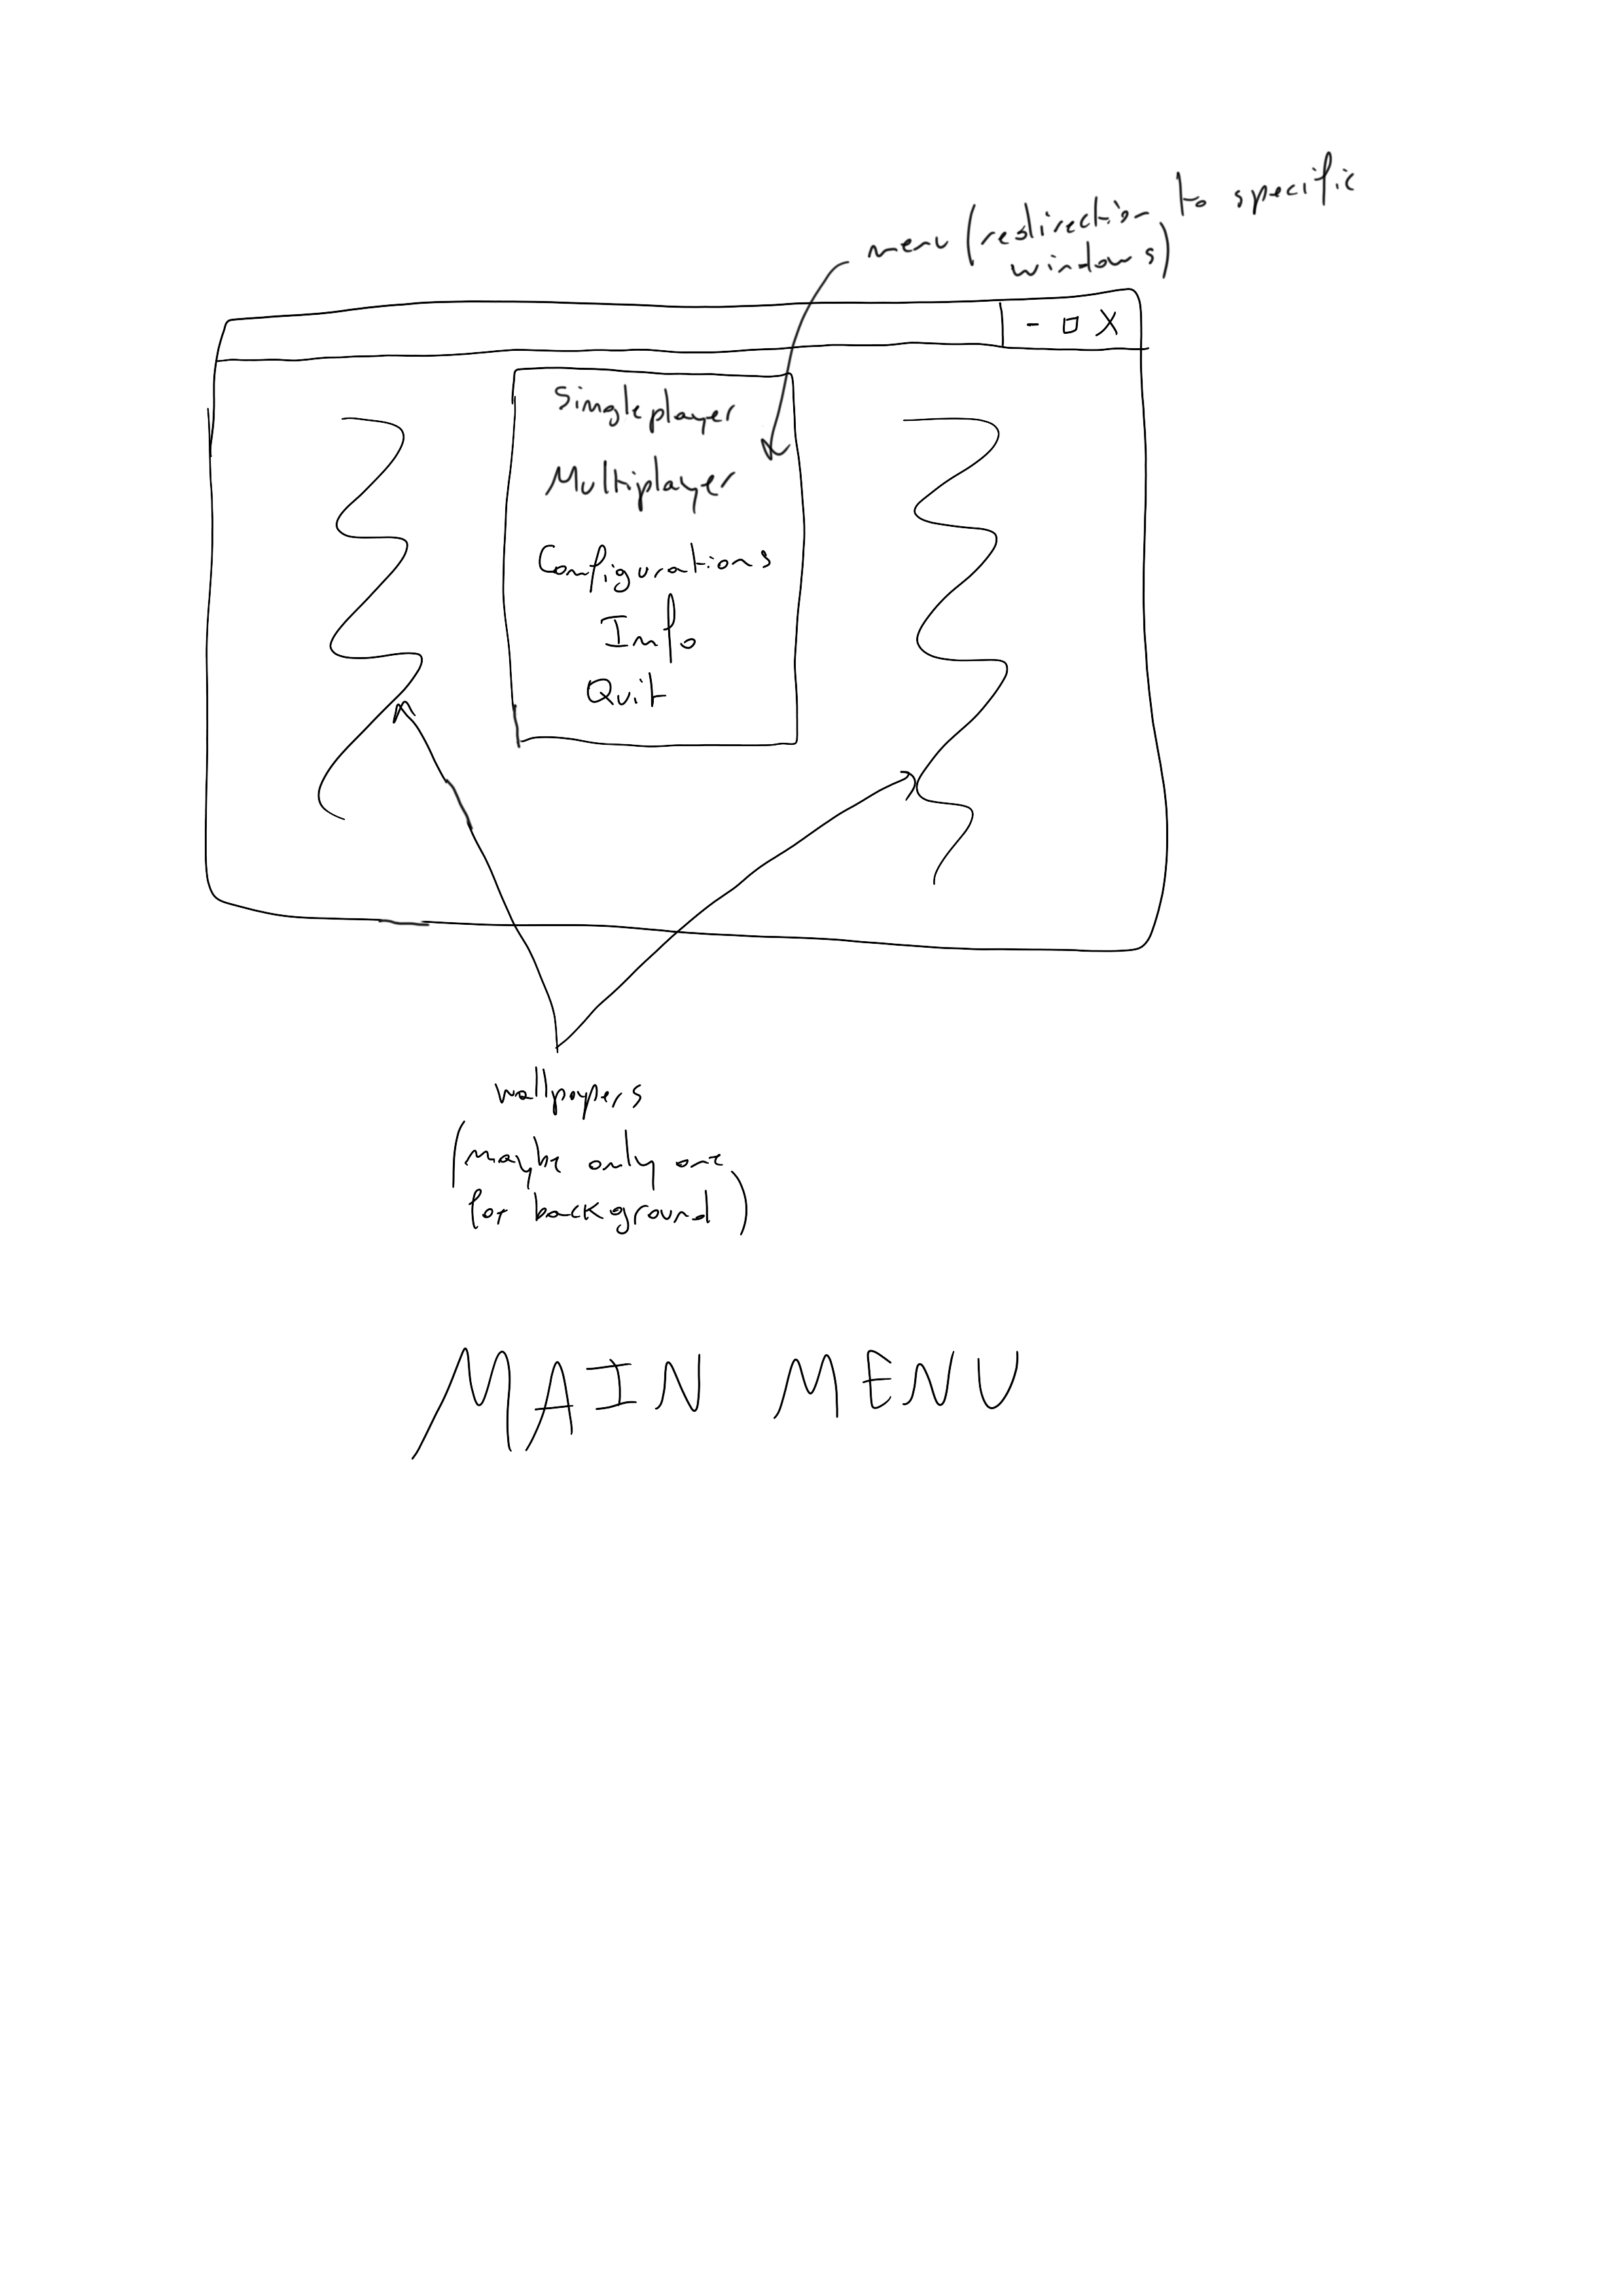
\includegraphics[width=0.5\linewidth, cfbox=blue 2pt 0pt]{GUI_schemas/main_menu_pdp.png}
        \caption{Menu principal du jeu}
        \label{fig:guimainmenu}
    \end{figure}
    \begin{figure}
        \centering
        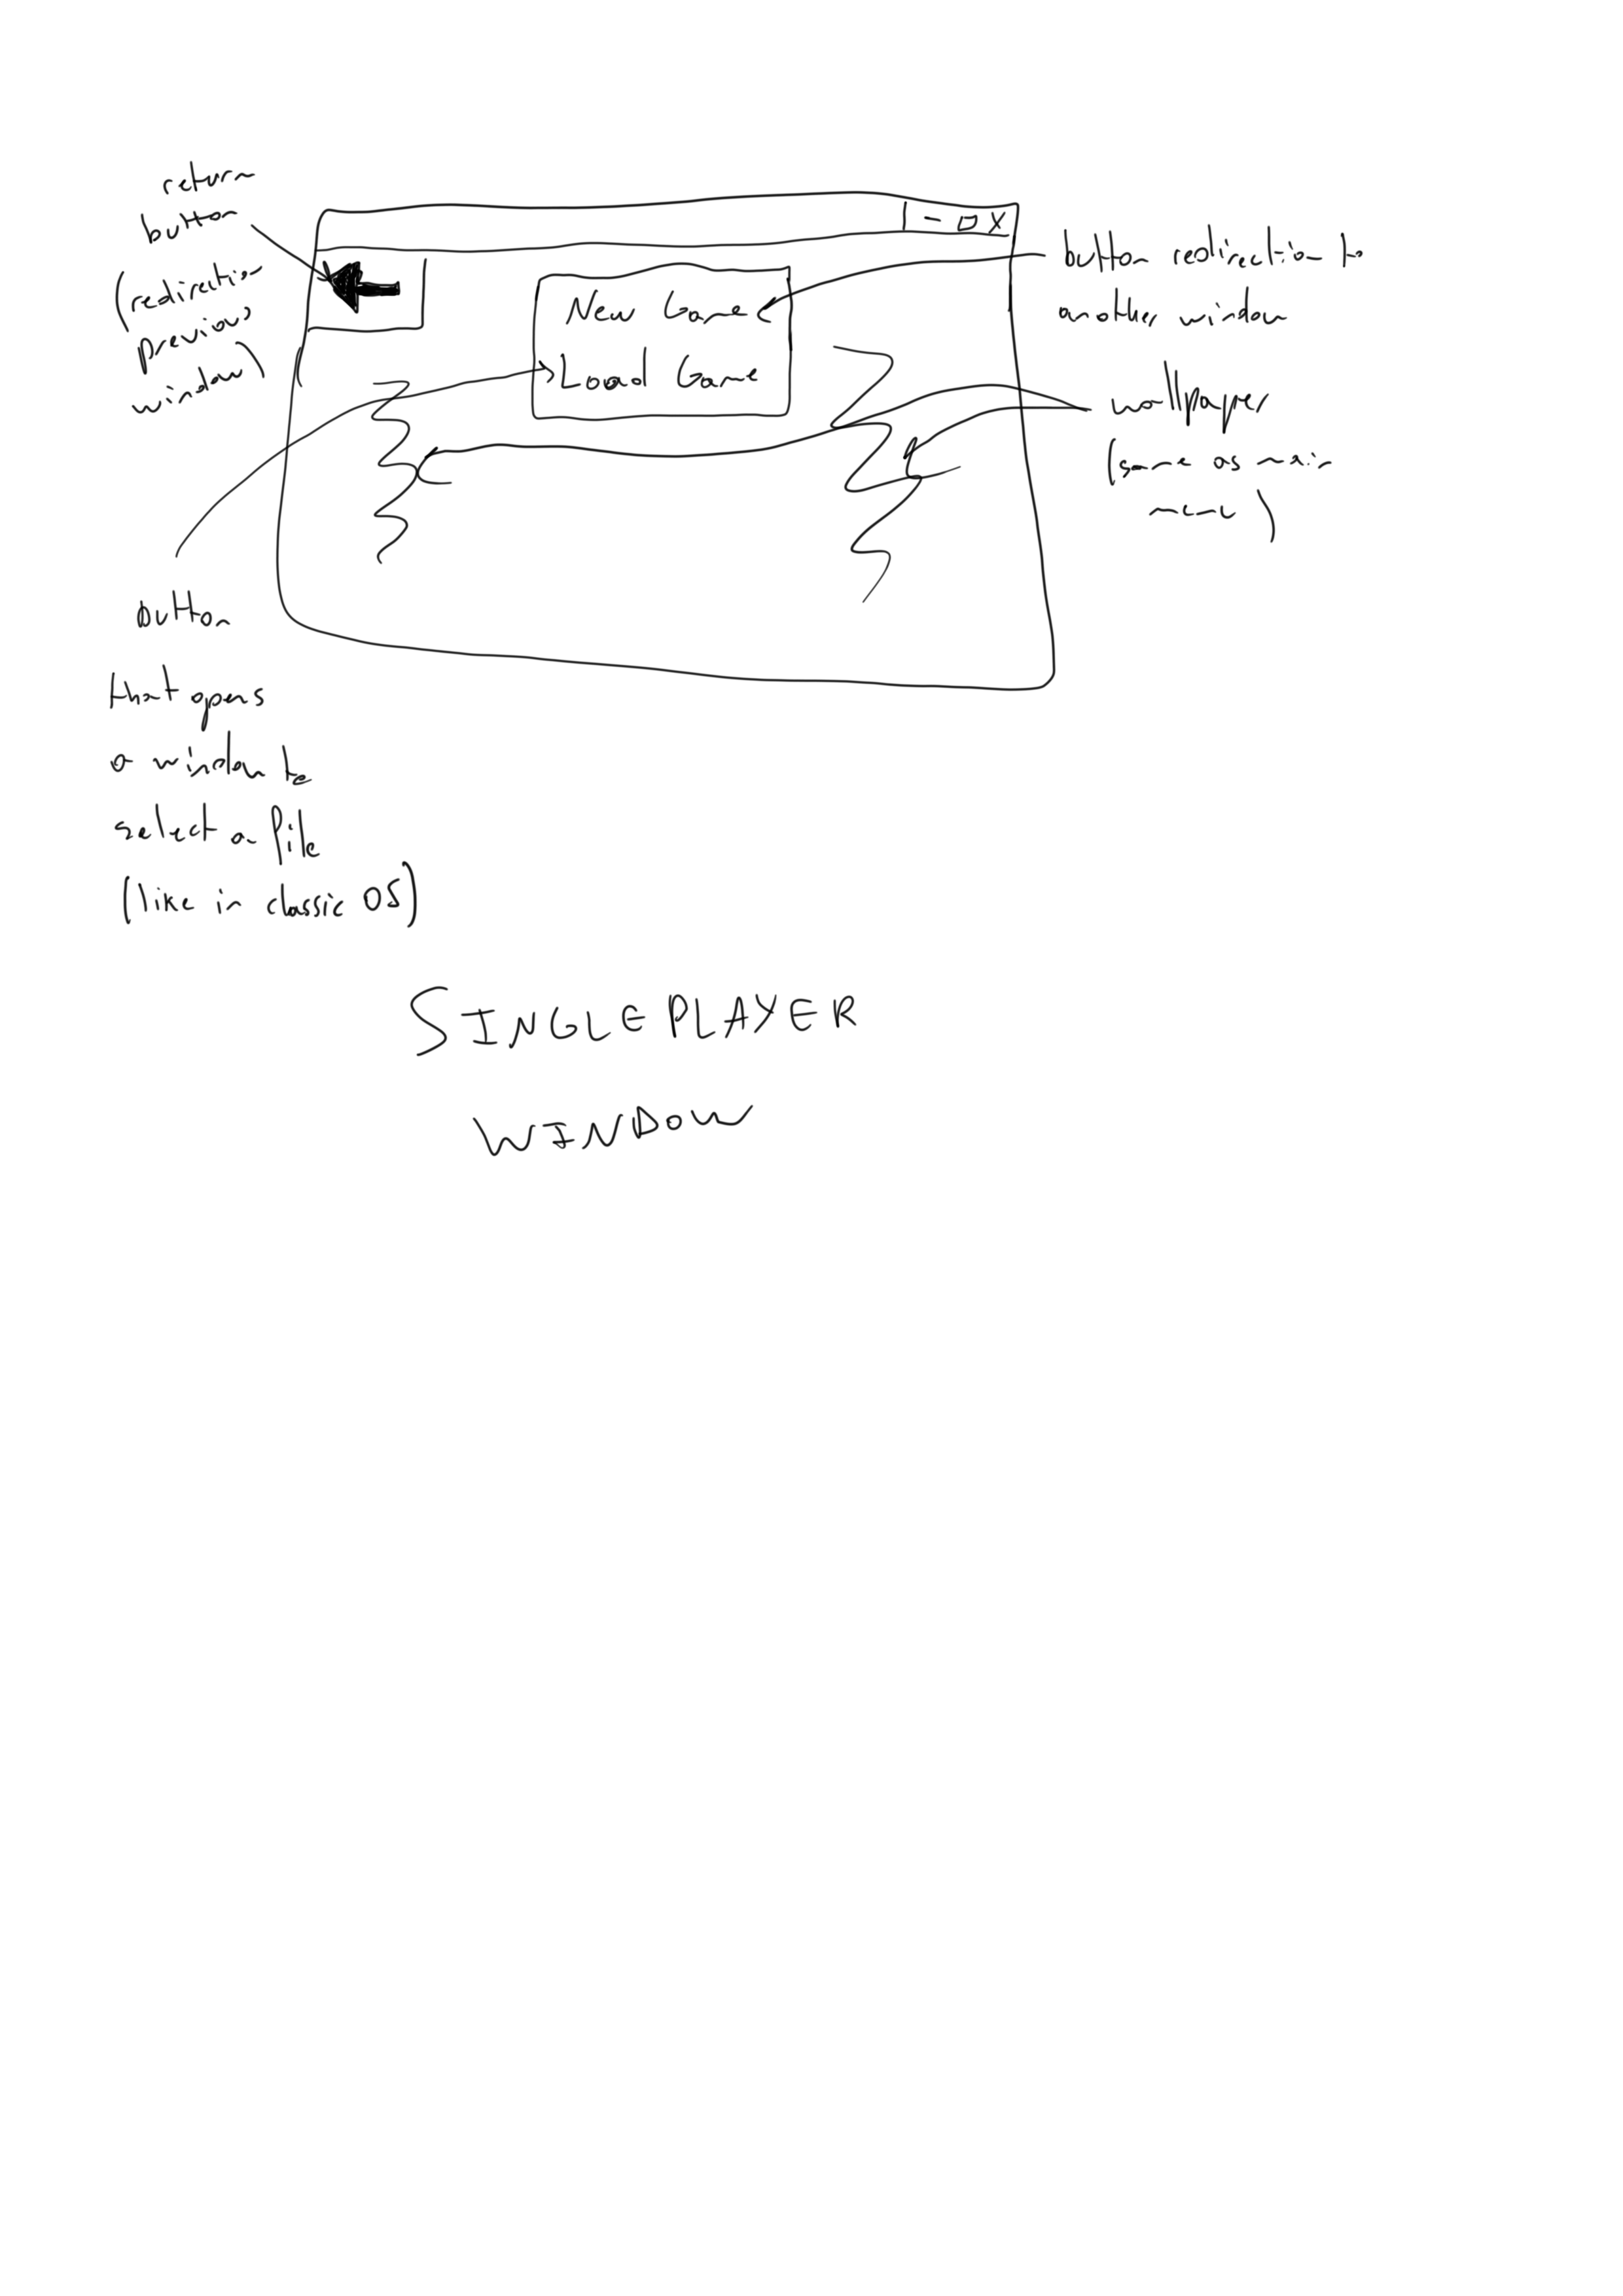
\includegraphics[width=0.5\linewidth, cfbox=blue 2pt 0pt]{GUI_schemas/singleplayer_pdp.png}
        \caption{Menu "singleplayer" du jeu}
        \label{fig:guisinglemenu}
    \end{figure}
    \begin{figure}
        \centering
        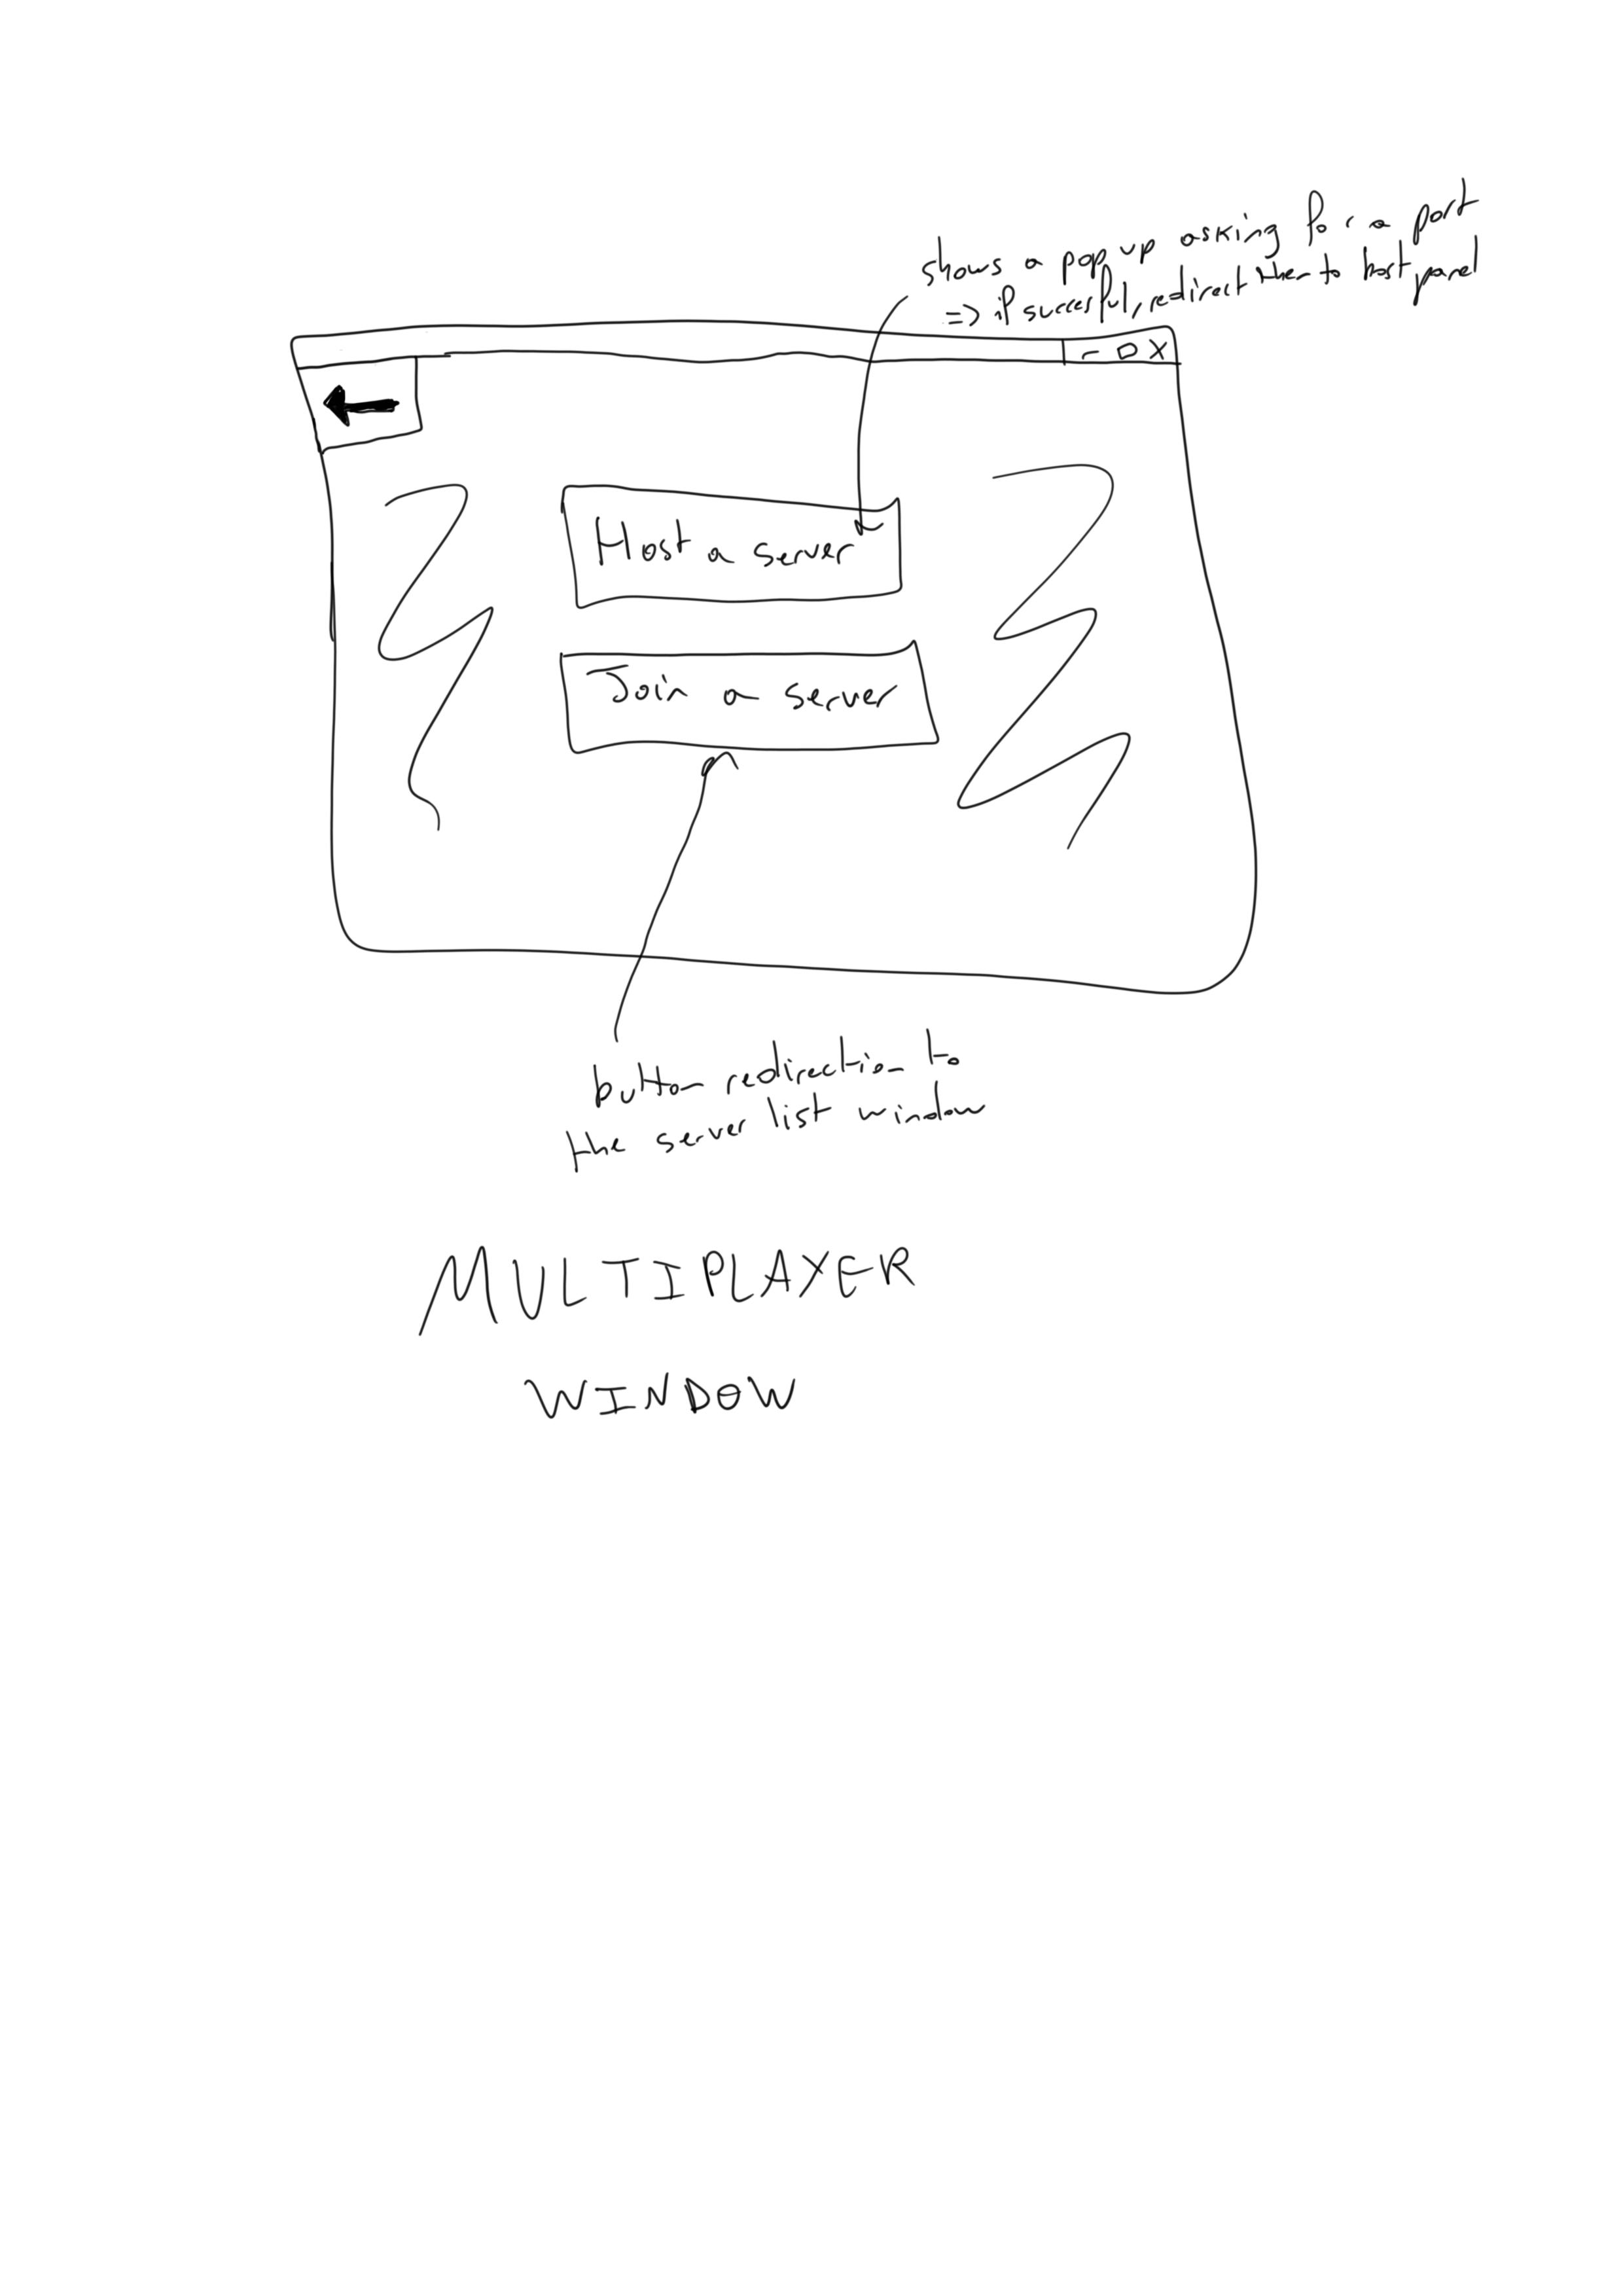
\includegraphics[width=0.5\linewidth, cfbox=blue 2pt 0pt]{GUI_schemas/multiplayer_pdp.png}
        \caption{Menu "multiplayer" du jeu}
        \label{fig:guimultimenu}
    \end{figure}
    \begin{figure}
        \centering
        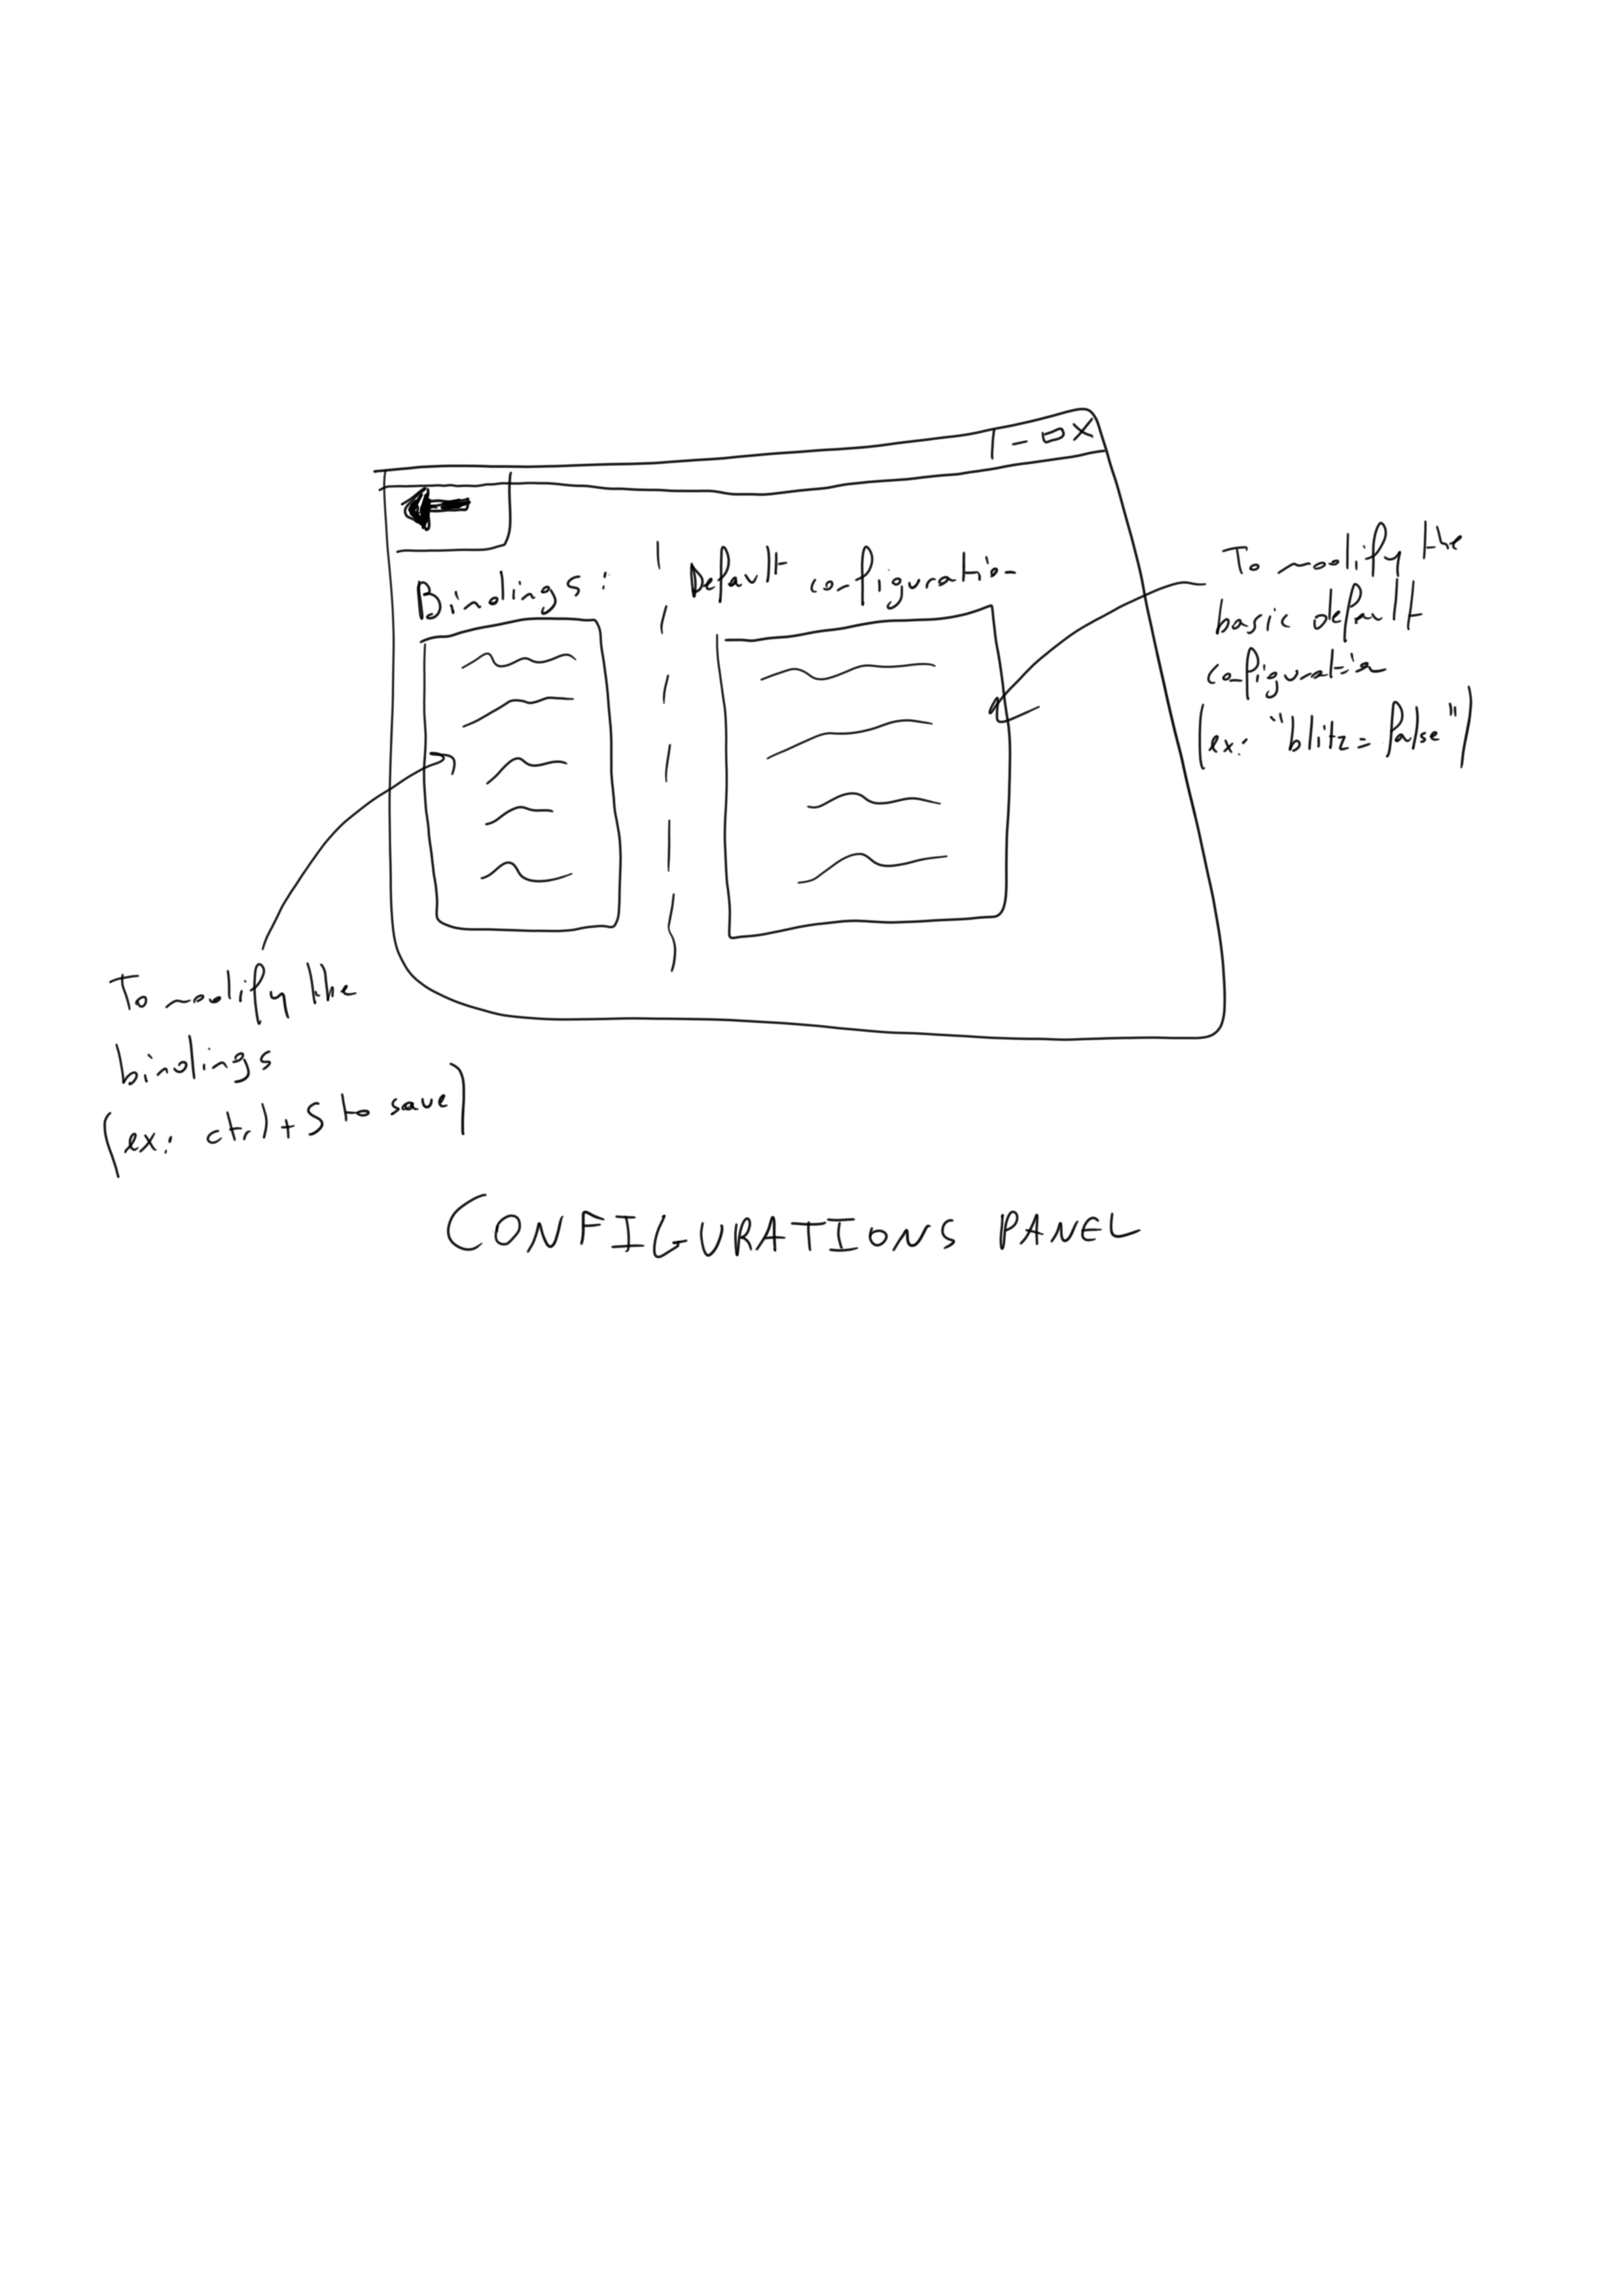
\includegraphics[width=0.5\linewidth, cfbox=blue 2pt 0pt]{GUI_schemas/config_panel_pdp.png}
        \caption{Configuration}
        \label{fig:guiconfig}
    \end{figure}
    \begin{figure}
        \centering
        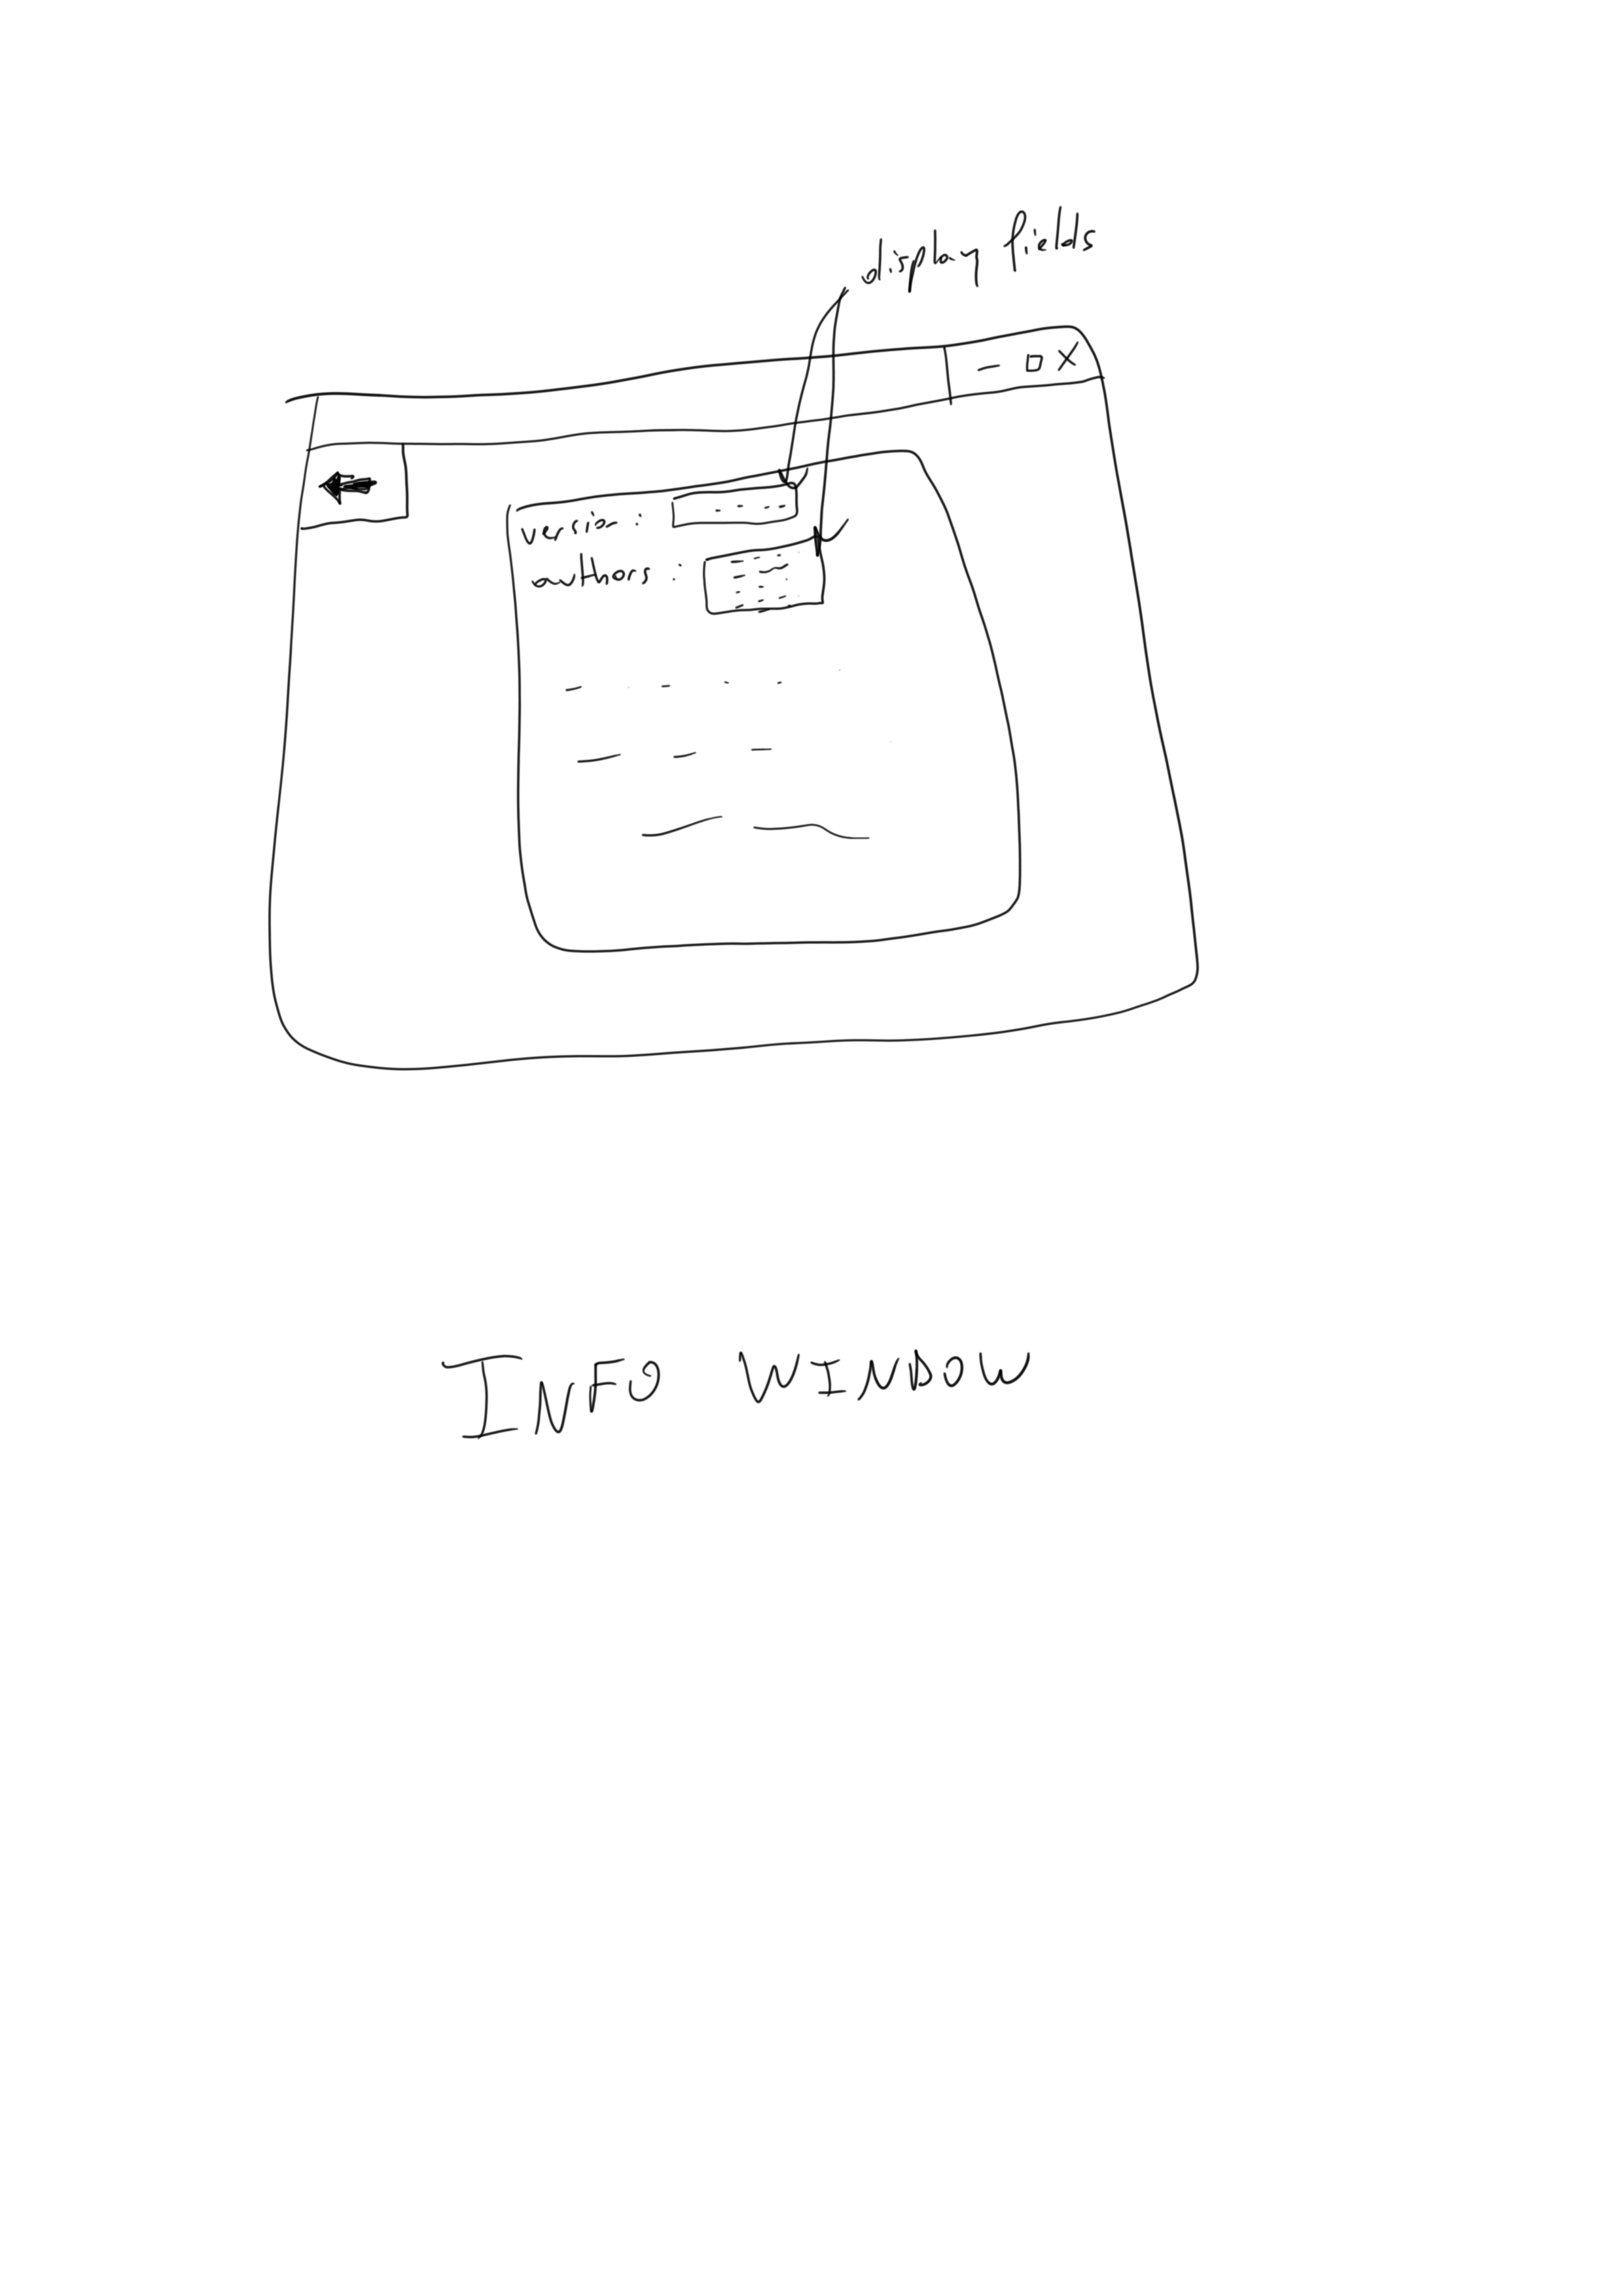
\includegraphics[width=0.5\linewidth, cfbox=blue 2pt 0pt]{GUI_schemas/info_pdp.png}
        \caption{Informations}
        \label{fig:guiinfo}
    \end{figure}
    \begin{figure}
        \centering
        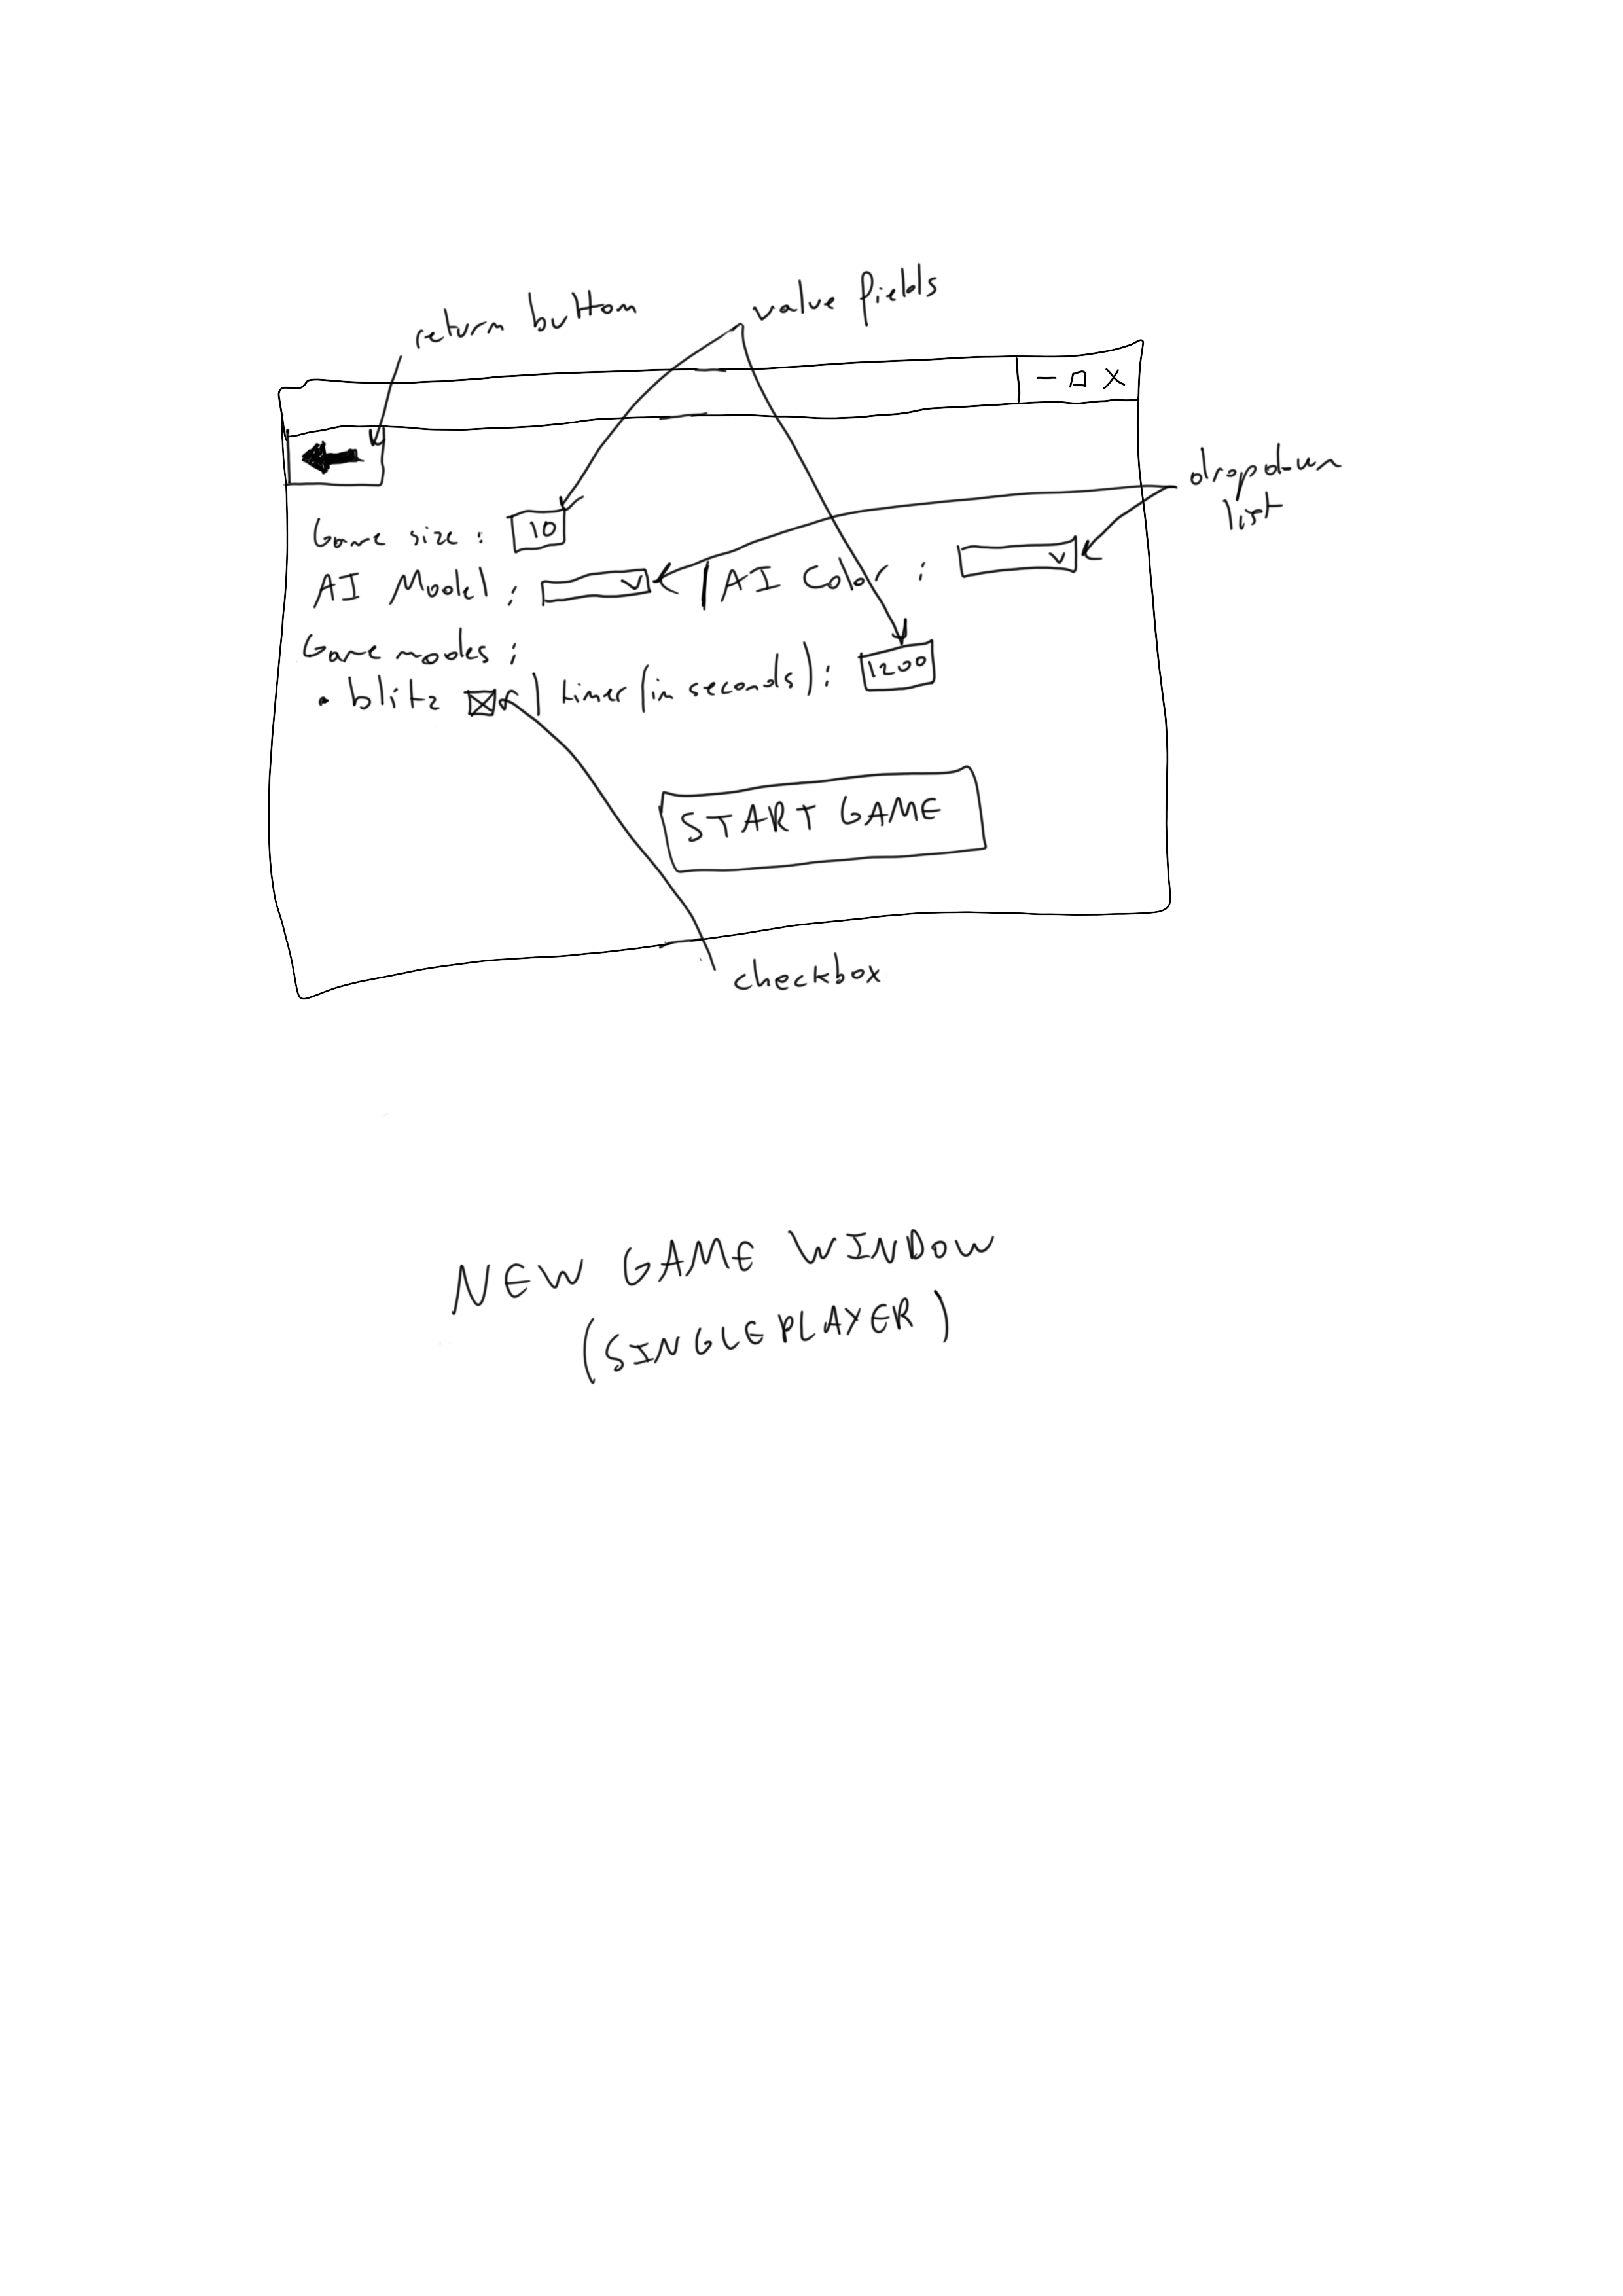
\includegraphics[width=0.5\linewidth, cfbox=blue 2pt 0pt]{GUI_schemas/new_game_pdp.png}
        \caption{Menu "Nouvelle partie"}
        \label{fig:guinewgame}
    \end{figure}
    \begin{figure}
        \centering
        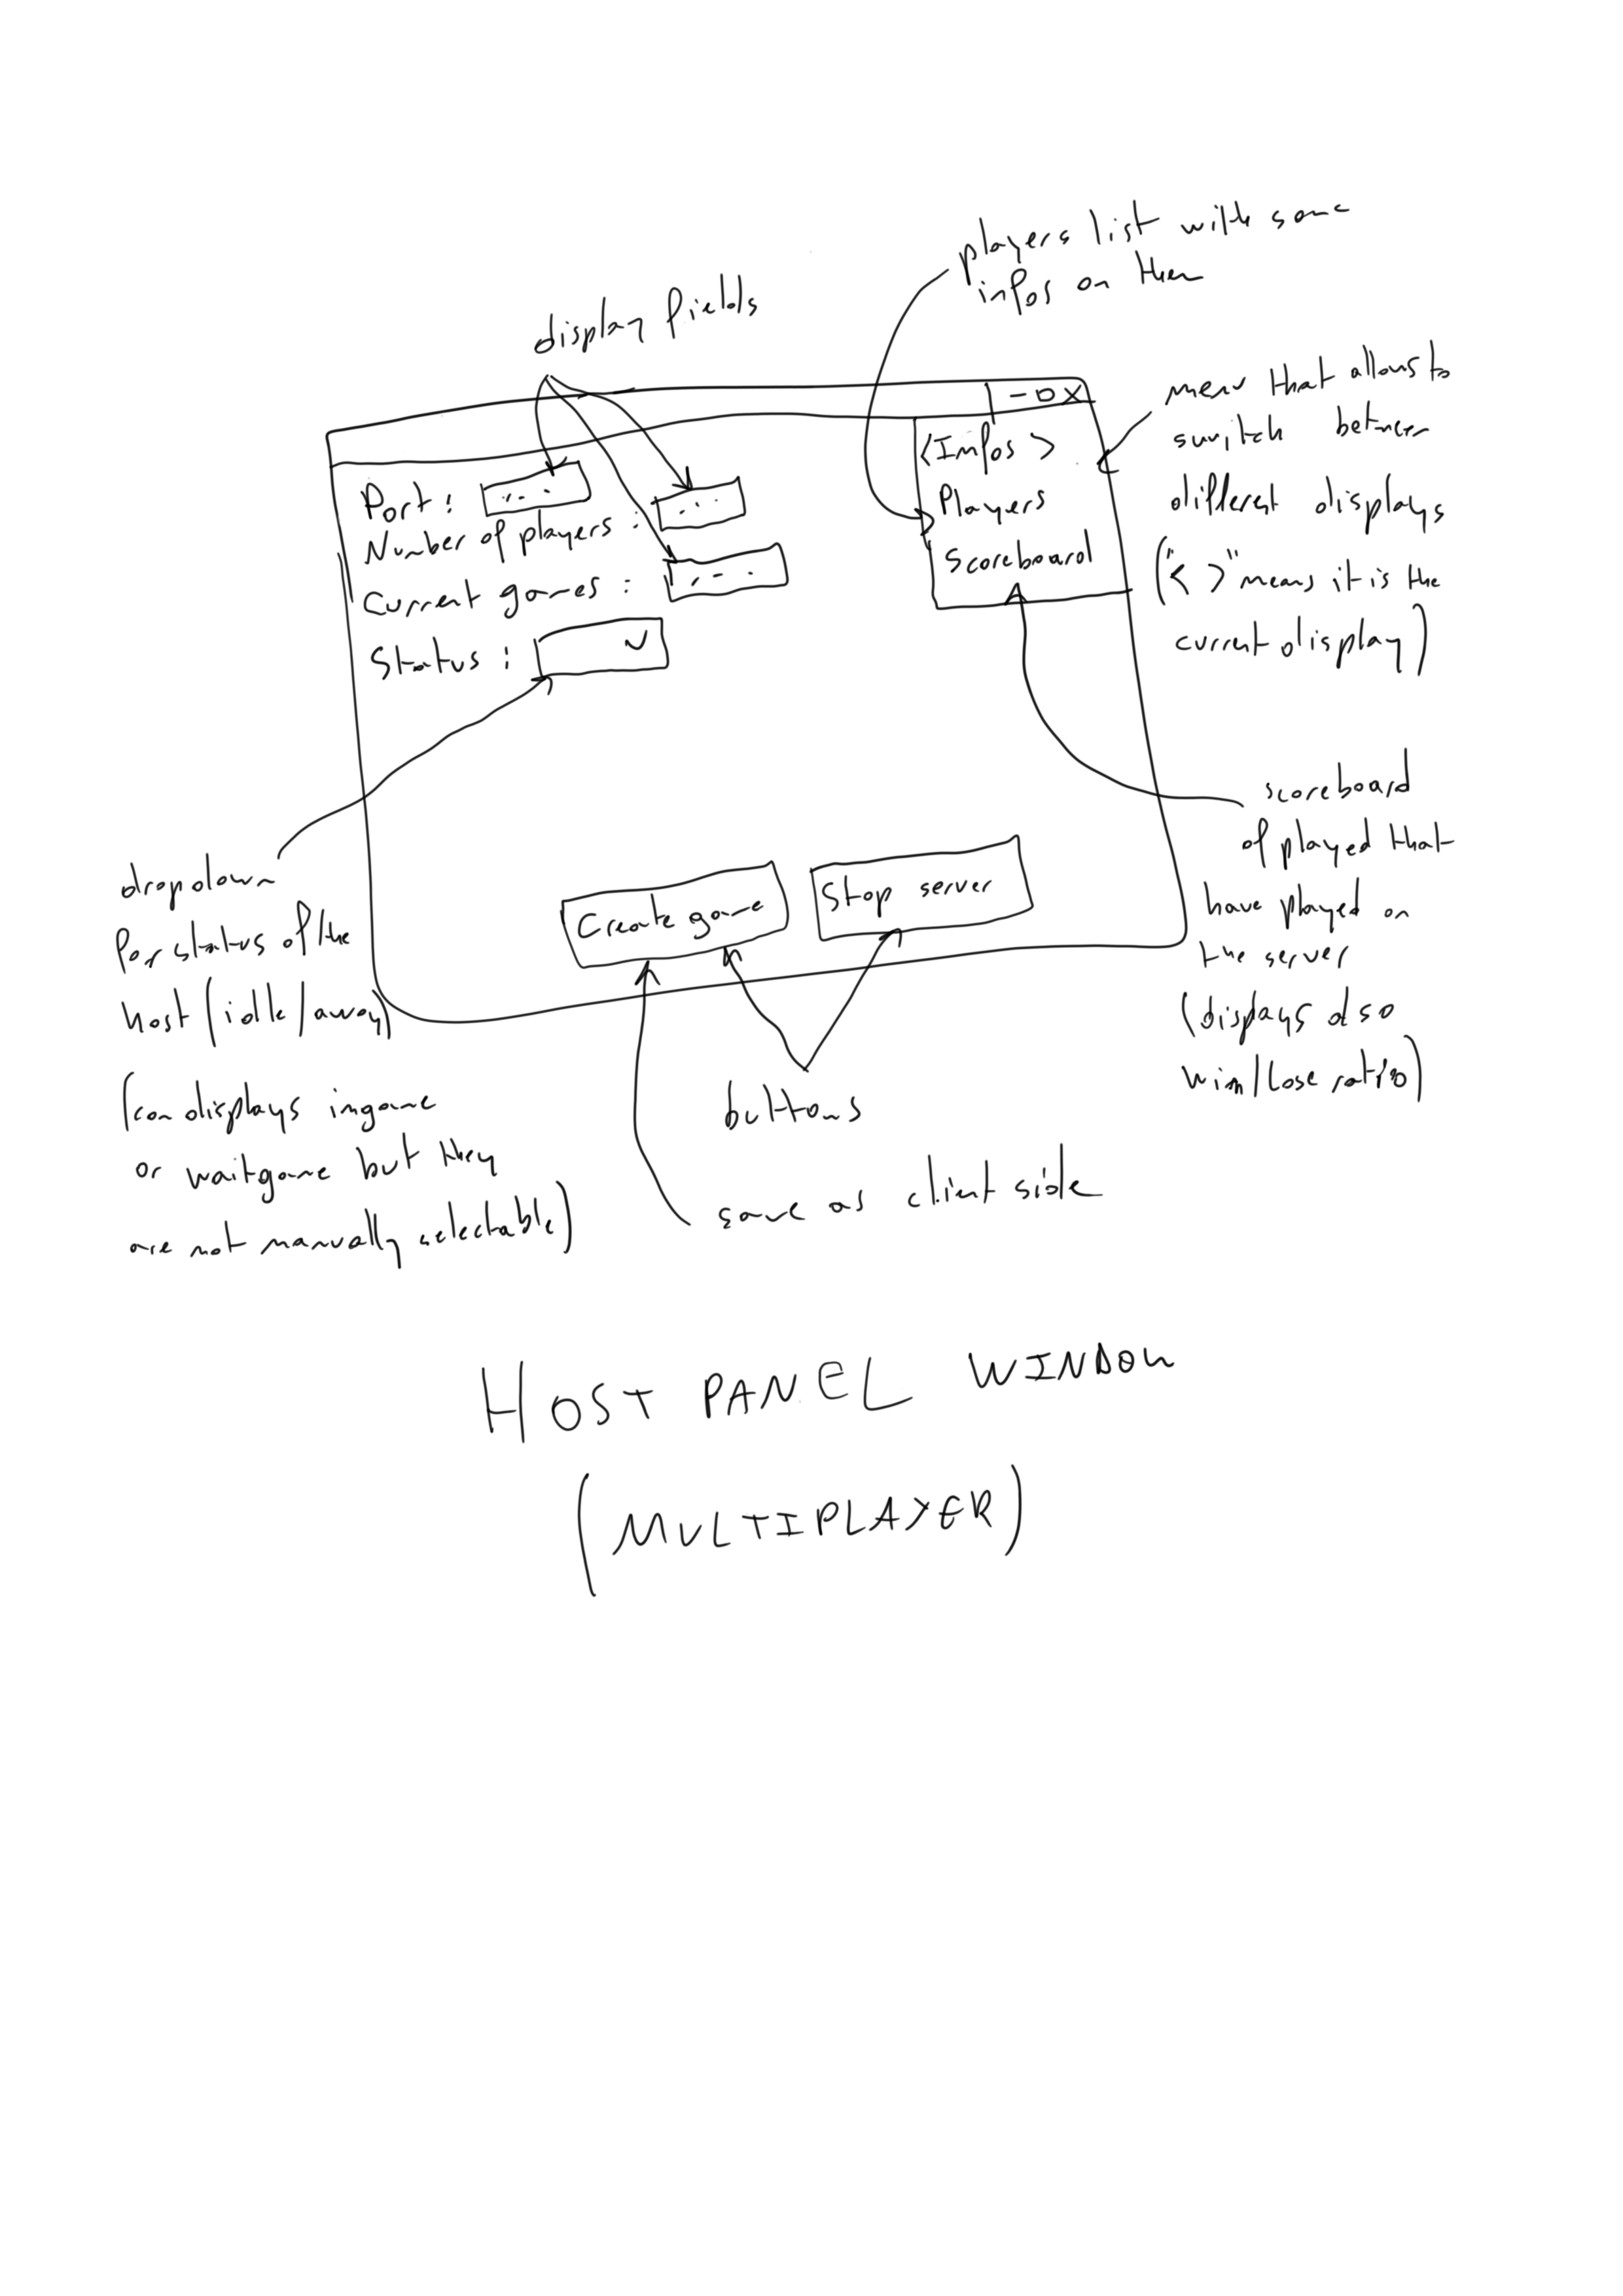
\includegraphics[width=0.5\linewidth, cfbox=blue 2pt 0pt]{GUI_schemas/host_panel_pdp.png}
        \caption{Menu du host}
        \label{fig:guihost}
    \end{figure}
    \begin{figure}
        \centering
        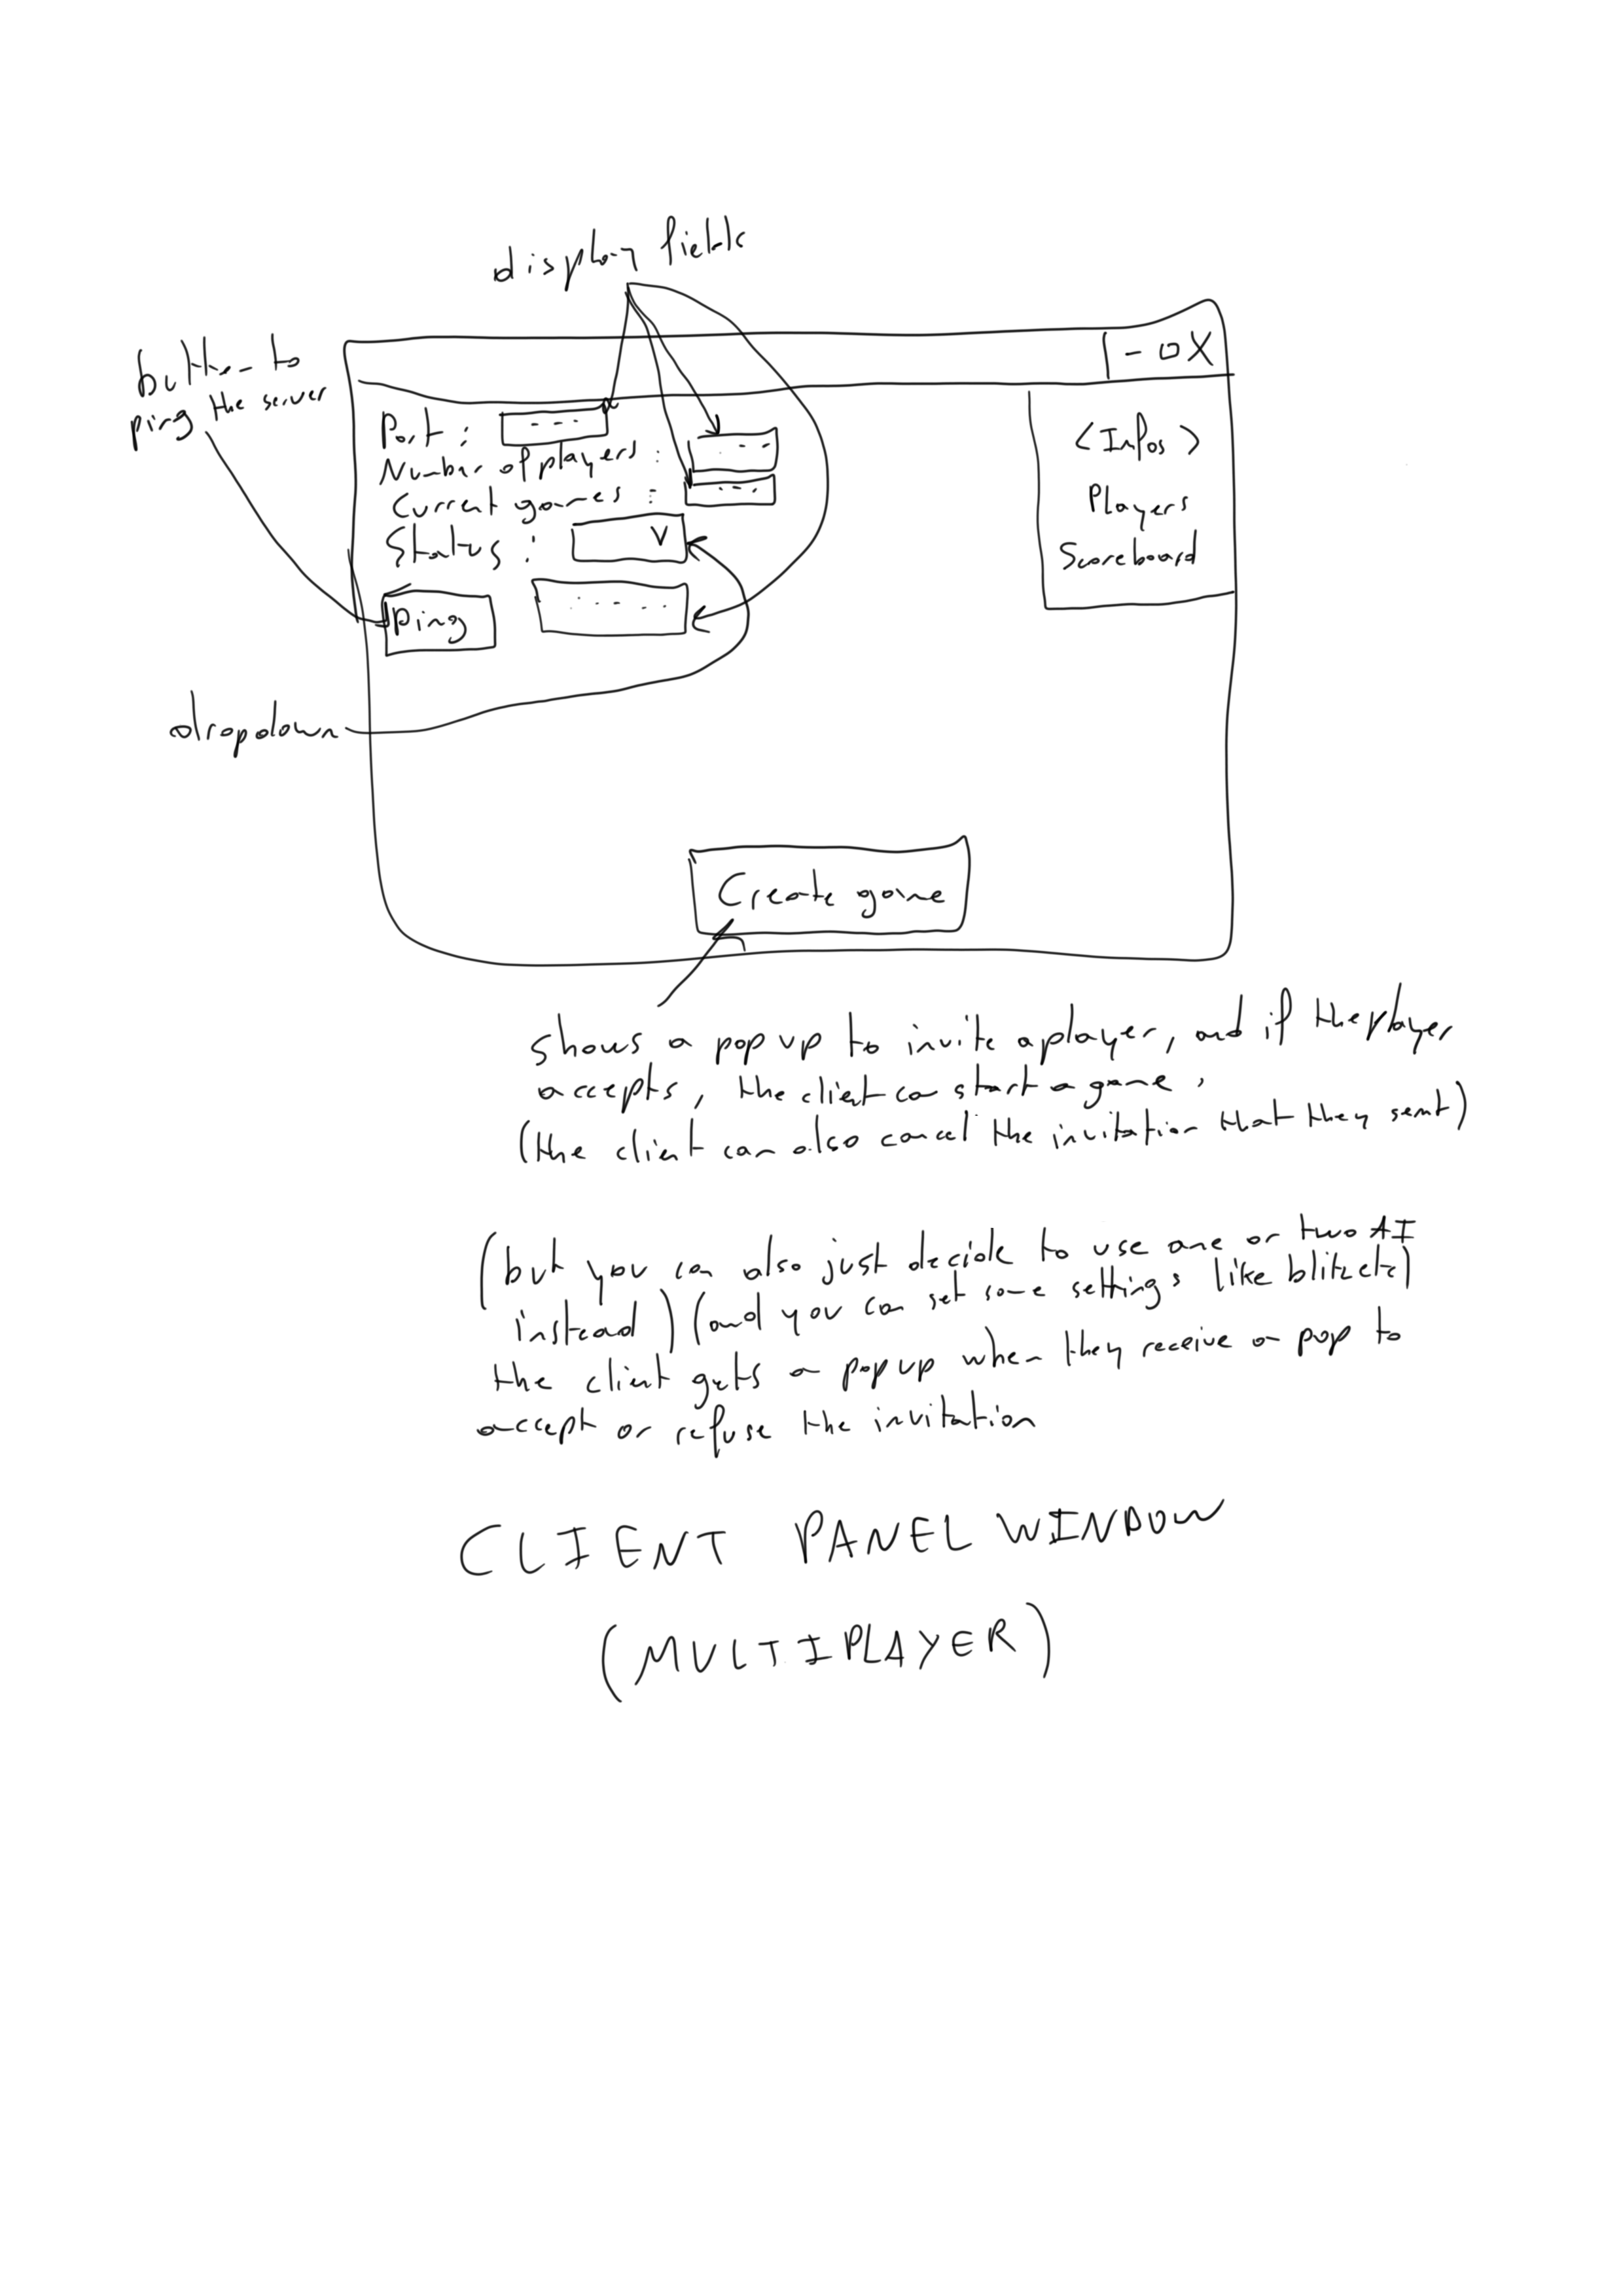
\includegraphics[width=0.5\linewidth, cfbox=blue 2pt 0pt]{GUI_schemas/client_panel_pdp.png}
        \caption{Menu du client}
        \label{fig:guiclient}
    \end{figure}
    \begin{figure}
        \centering
        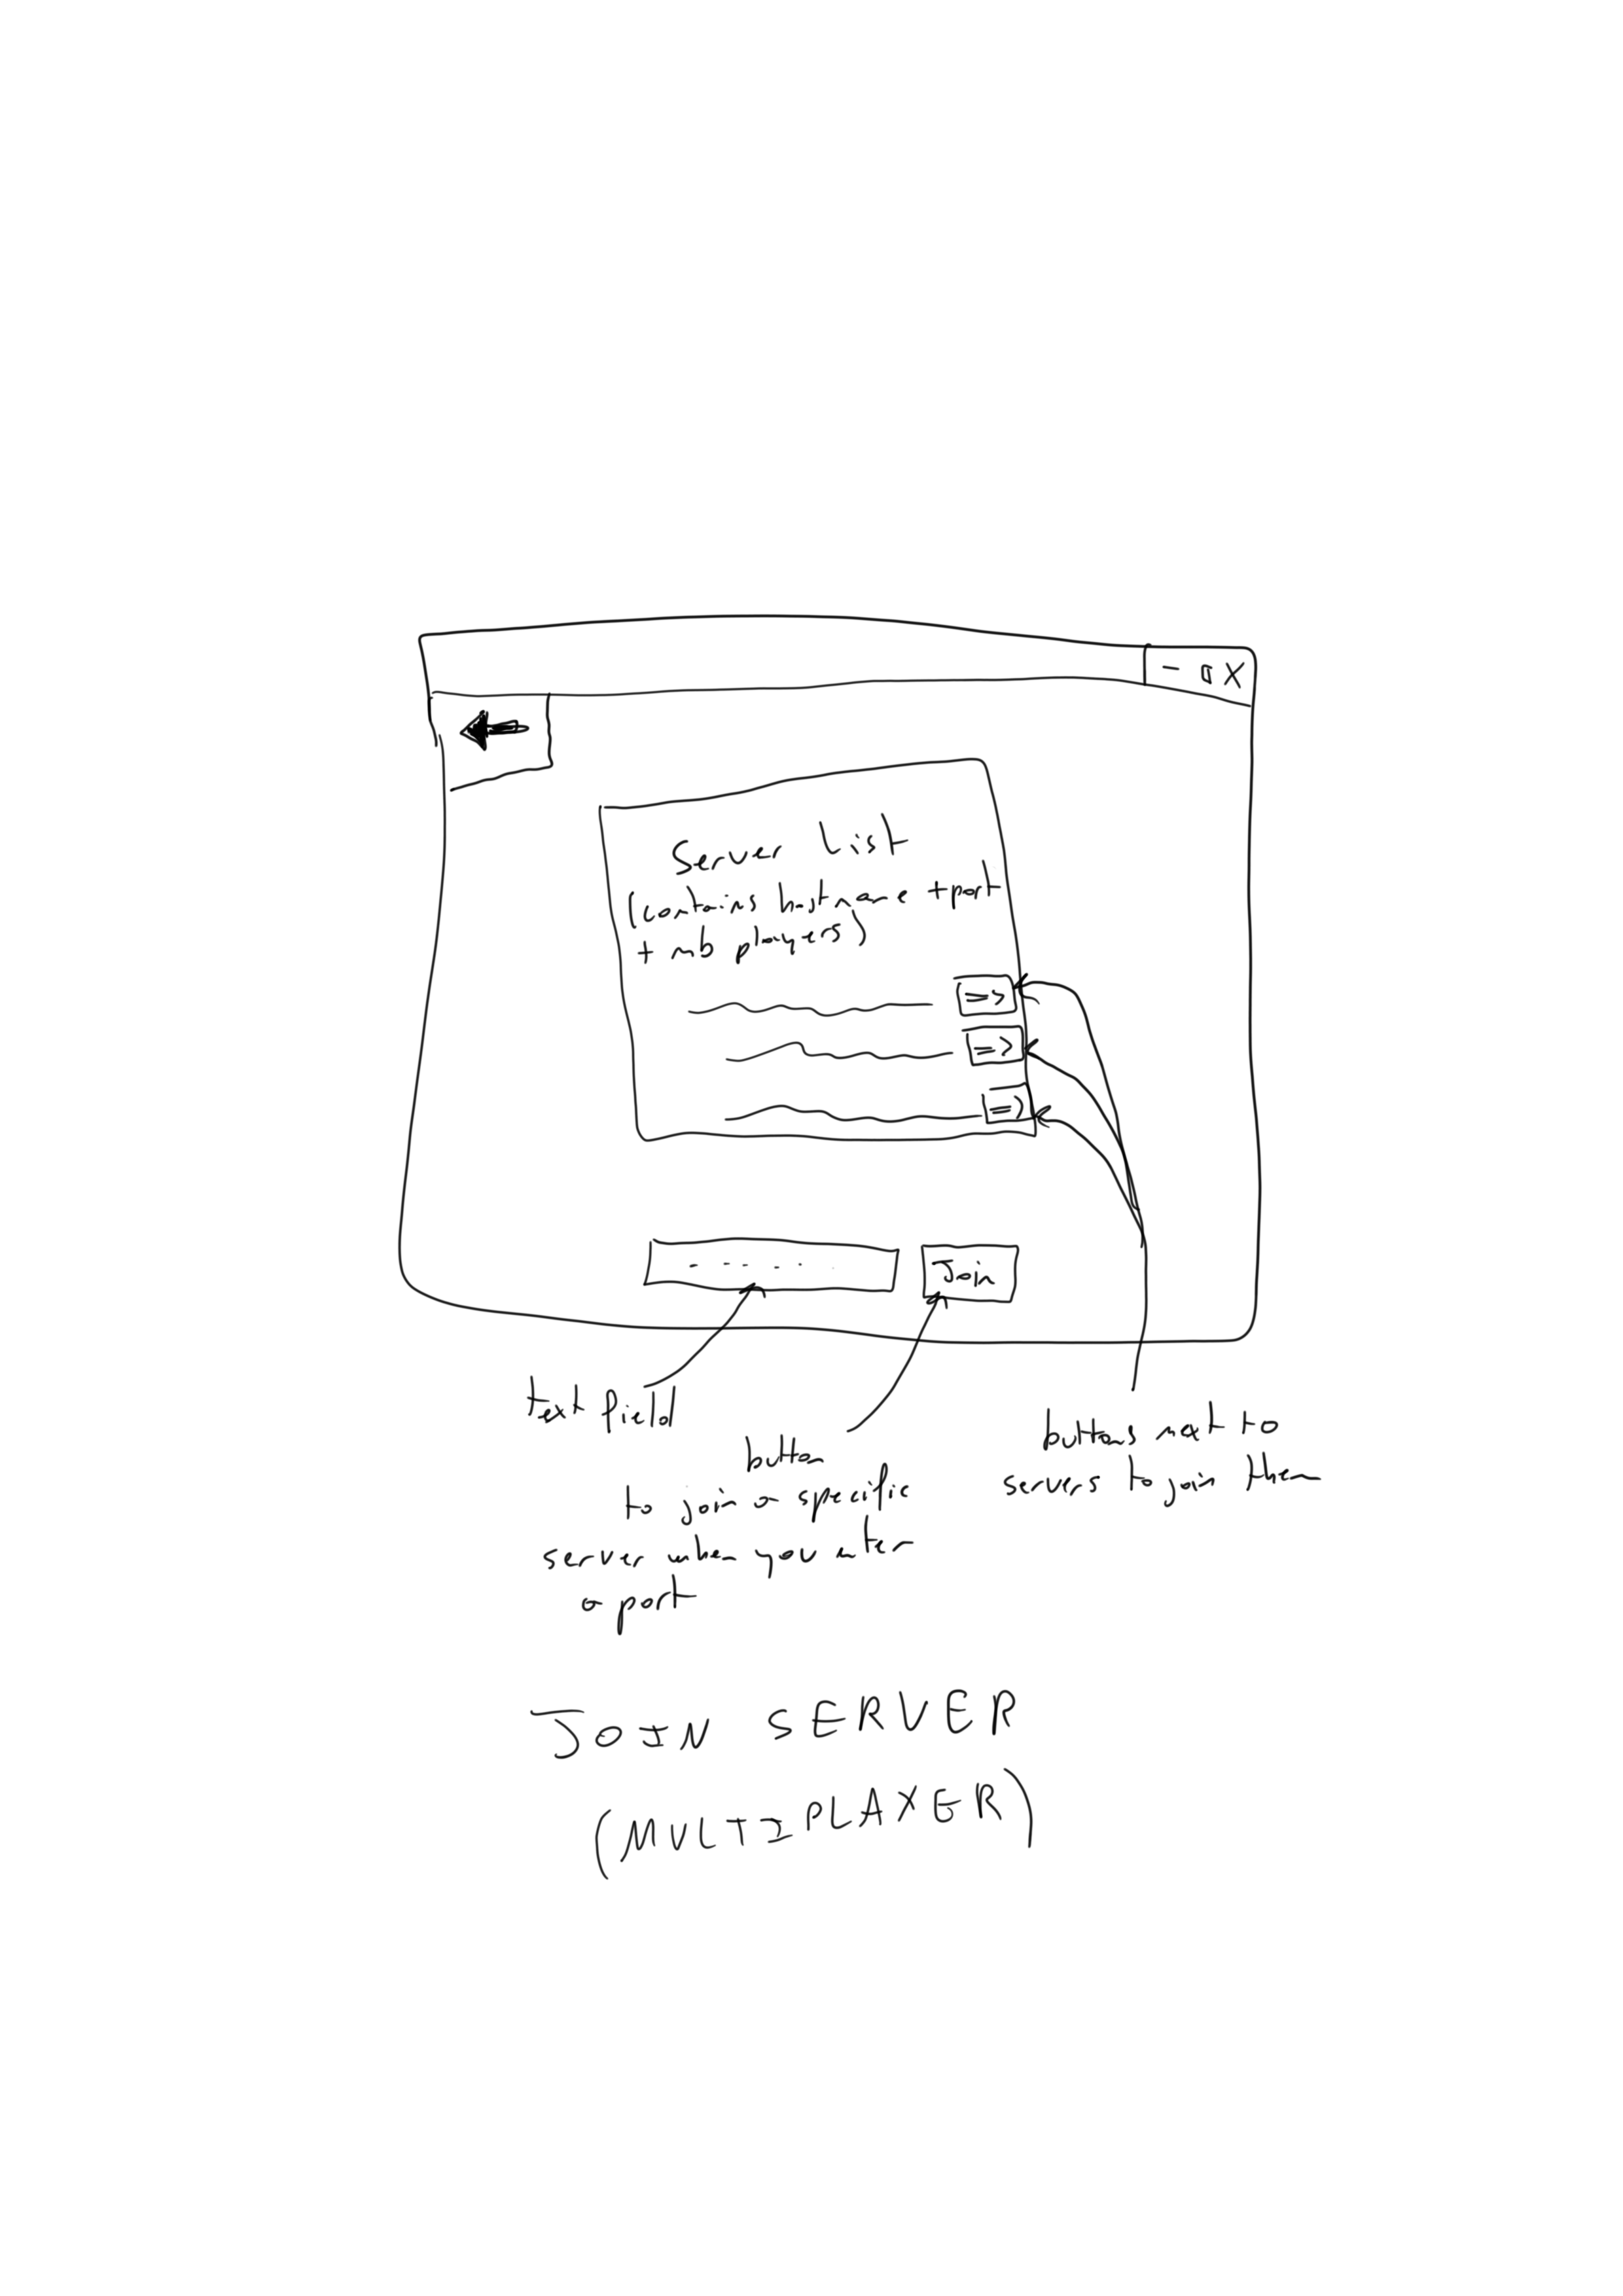
\includegraphics[width=0.5\linewidth, cfbox=blue 2pt 0pt]{GUI_schemas/join_server_pdp.png}
        \caption{Liste des serveurs}
        \label{fig:guiservlist}
    \end{figure}
    \begin{figure}
        \centering
        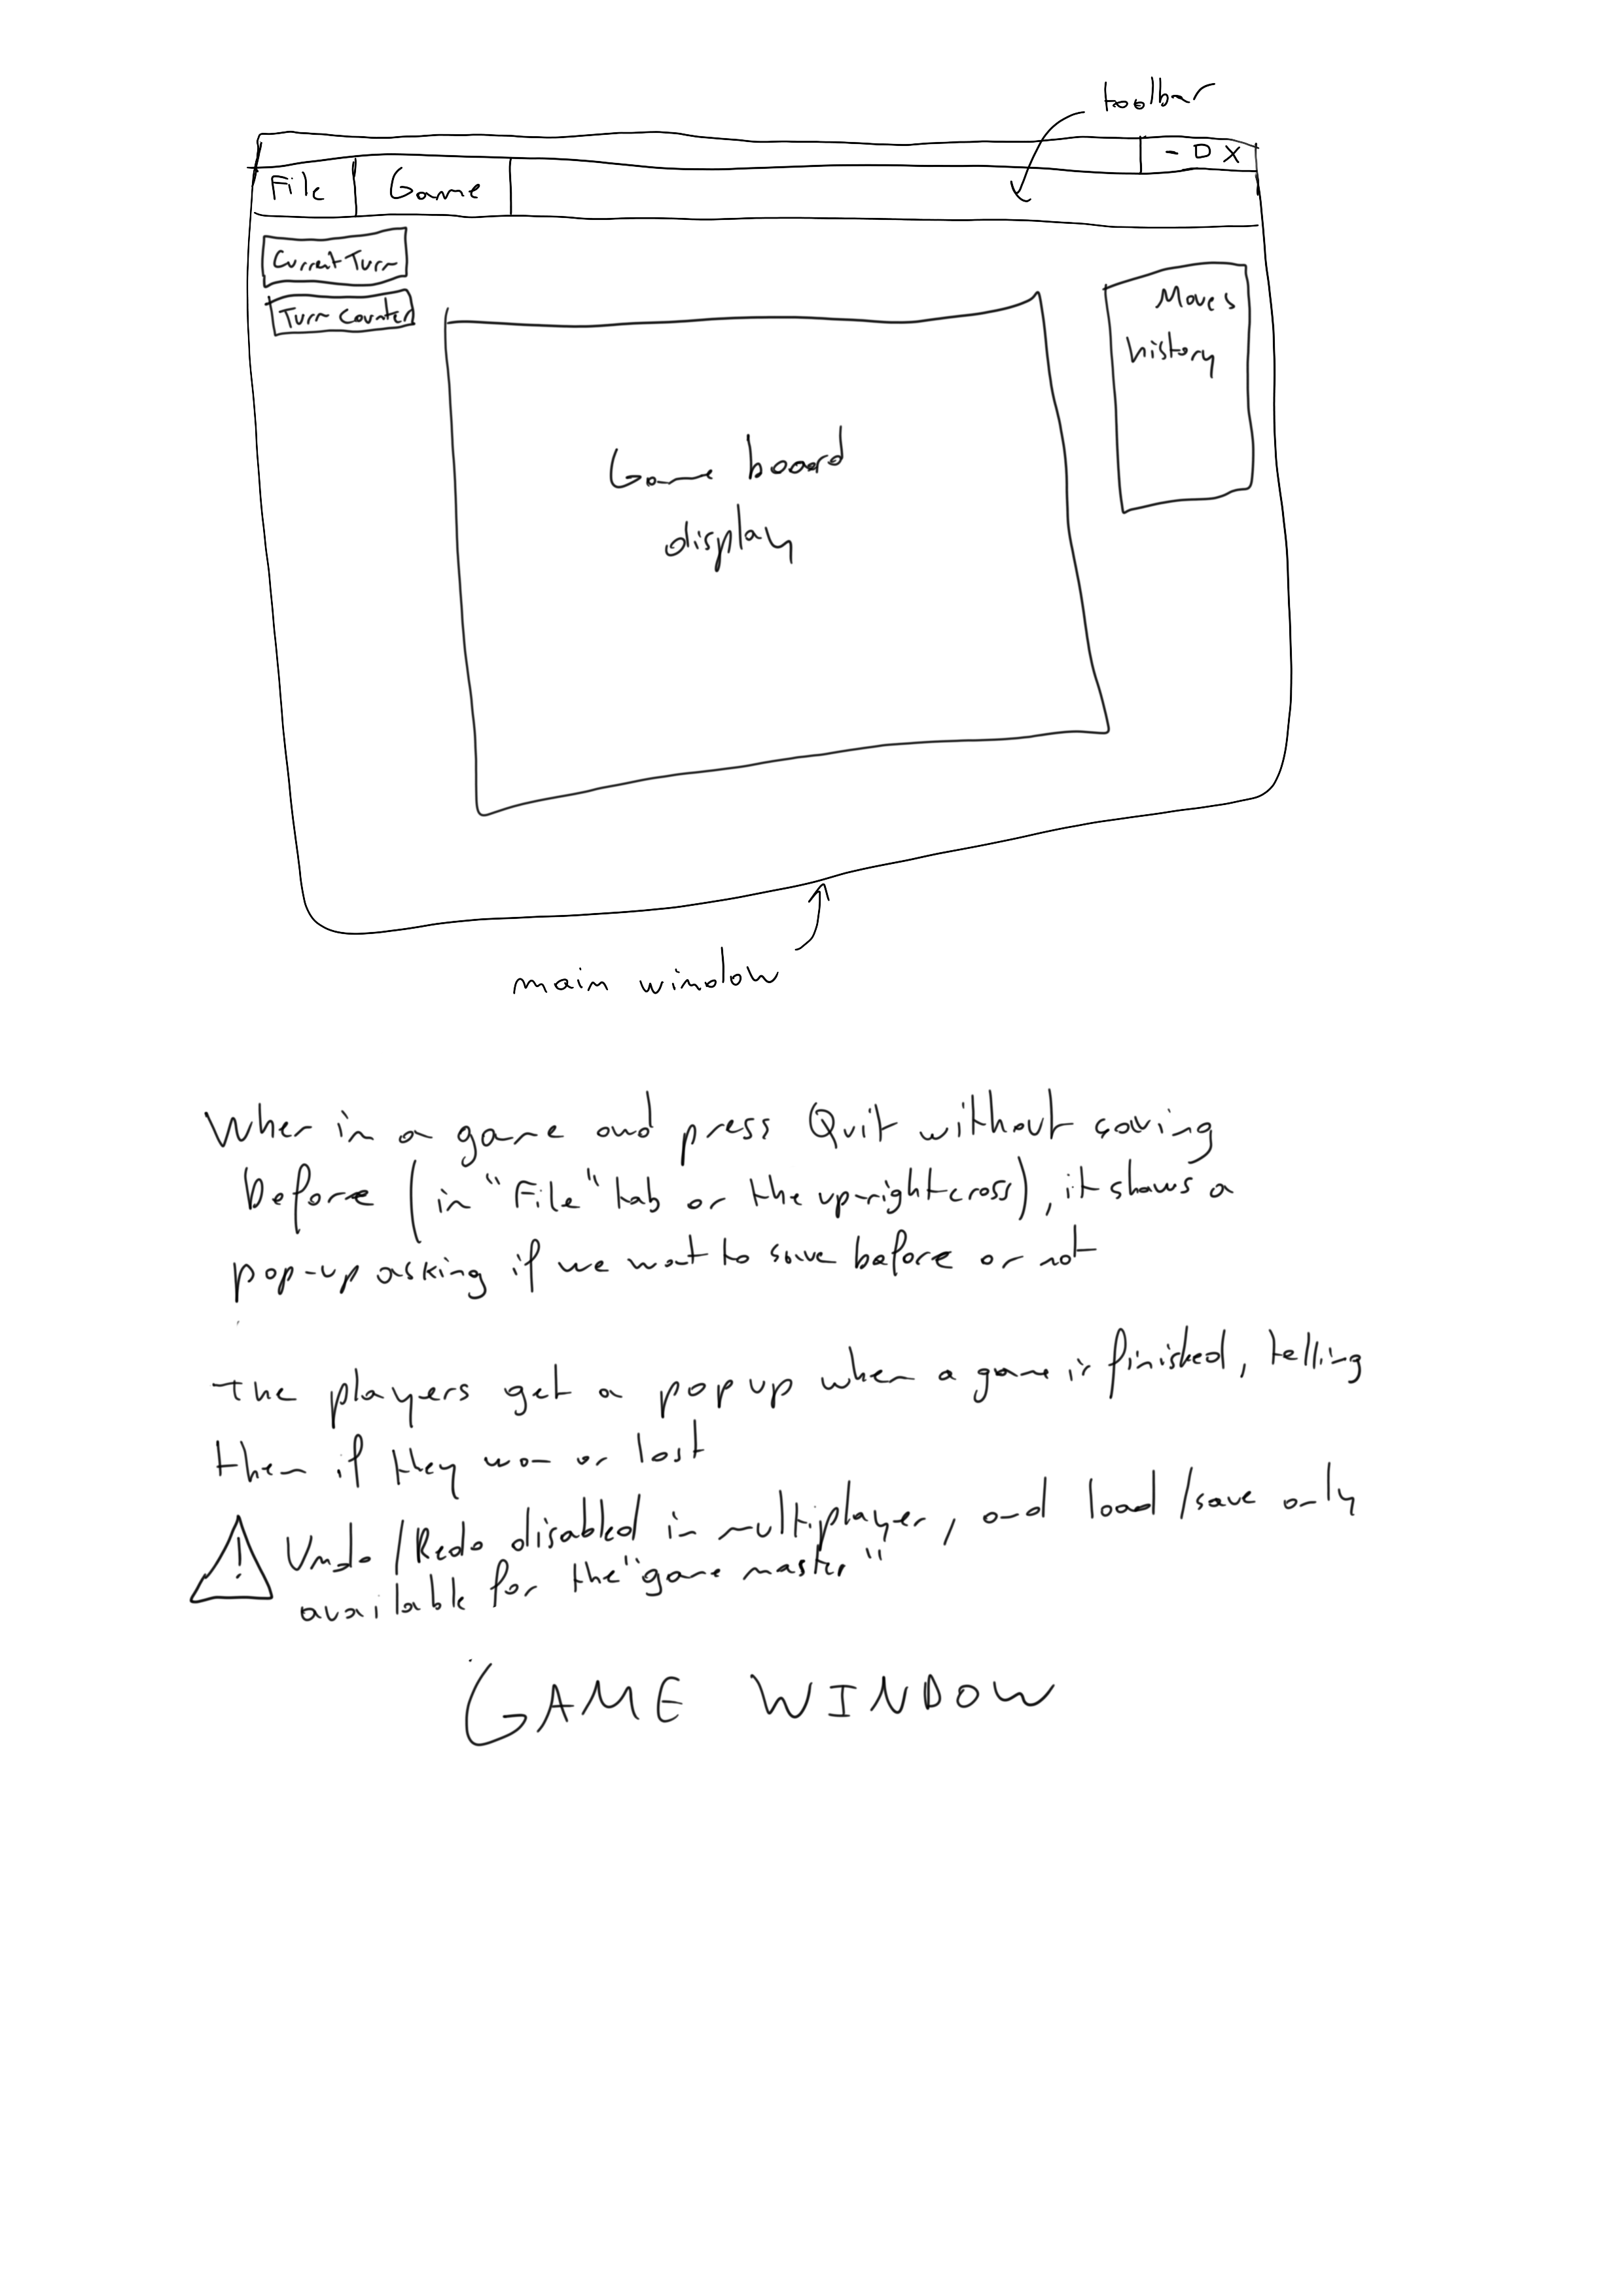
\includegraphics[width=0.5\linewidth, cfbox=blue 2pt 0pt]{GUI_schemas/game.pdp.png}
        \caption{Fenêtre du jeu}
        \label{fig:guigame}
    \end{figure}

    Gtk utilise une application principale (GtkApplication) comme structure. On peut ensuite y rajouter des éléments comme GtkButton pour gérer un système de boutons (lancer une partie, quitter le jeu, ...), GtkWidget pour construire différents modules interactifs (des listes, des affichages particuliers, ...) et également GtkStack pour permettre "d'empiler des pages" et ainsi fluidifier le changement de fenêtre (en réalité cela simule un changement de fenêtre, mais c'est justement l'avantage de GtkStack, on a une transition fluide entre le menu principal du jeu et le menu "singleplayer" par exemple.
    
    De plus, Gtk offre la possibilité d'intégrer du Drag'n'Drop (pour déplacer les pions par exemple) grâce à GtkDragSource et GtkDropTarget. 
    
    \subsection{Intégration et CLI}
    Le module d'intégration est le pilier central de l'application. Pour garantir un code propre et éviter d'éparpiller les données dans des variables globales, nous avons regroupé tout l'état de l'application dans une structure centrale nomée \texttt{Application}.
    Cette structure contient toutes les dépendances du programme. Elle gère trois aspects essentiels : 
    \begin{itemize}
        \item \textbf{GameConfig :} Elle contient la configuration du jeu et les paramètres immuables(mode verbeux, port réseau ...) chargés au lancement.
        \item \textbf{GameEngine* :} Un pointeur vers l'instance unique du moteur de jeu.
        \item \textbf{Contrôle de flux :} Des drapeaux atomiques (ex: \begin{verbatim}is_running\end{verbatim}) permettant une terminaison propre et la libération des ressources via une procédure de nettoyage.
    \end{itemize}
    En parallèle, pour découpler la saisie utilisateur de l'exécution, nous utilisons une structure \texttt{UserCommand}. Elle normalise les entrées : une commande textuelle brute transformée en un type énuméré, accompagné d'arguments validés, facilitant le travail du Dispatcher.
    

    \section{Algorithmes utilisés} 
    \subsection{Réseaux}
    Bien que le projet ne nécessite pas d'algorithmes complexes en réseau, la robustesse du module repose sur trois algorithmes système fondamentaux que nous voulons implémenter :
    \begin{itemize}
        \item On utiliserais un algorithme de reconstruction TCP qui accumulerais les données brutes dans un buffer persistant jusqu'à détecter un caractère de fin de message, puis extrairais la commande complète pour traiter la fragmentation des messages.
        \item Un algorithme de multiplexage qui utiliserais poll() pour surveiller simultanément l'activité du clavier, du serveur et des clients avec un temps d'attente nul affin d'éviter les opération bloquantes.
        \item Enfin on utiliserais  un algorithme de Routage sélectif qui parcourerais la liste des clients et ne relaierais les messages qu'aux joueurs partageant le même "game id" que l'expéditeur pour éviter qu'un joueur ne reçoive les coups d'une autre partie en cours.
    \end{itemize}
    
    \subsection{IA}
    \subsubsection{Relative Territory Heuristic (RTH)}
        Bon je trouve pas comment la faire. Potentiellement à remplacer par territory-and-mobility (dispo sur https://project.dke.maastrichtuniversity.nl/games/files/msc/Hensgens\textunderscore thesis.pdf, où y en a plein.)
    \subsubsection{Queen Distance \& King Distance (QD\&KD)}    
    \subsubsection{Mobility Evaluation (ME)}
    \subsubsection{Monte Carlo Tree Search (MCTS)}
    \subsubsection{Upper Confidence bounds for Trees (UCT)}
    \subsubsection{Machine Learning (ML)}

    \subsection{Moteur de jeu}
        \subsubsection{Génération par Ray-Casting}

        L'algorithme de génération des coups doit gérer une complexité supérieure à celle des échecs en raison de la nature composée d'un tour(Déplacement + Tir). Nous utilisons une approche de "Ray-Casting" imbriqué.
        Dans un premier temps, l'algorithme projette les déplacements possibles de l'amazone selon les 8 axes. Pour chaque case d'arrivée valide, une seconde passe de rayons est lancée pour déterminer les cibles de flèches. Pour valider un tir, l'algorithme doit considérer la case de départ de l'amazone comme vide temporairement, car la flèche peut traverser l'ancienne position de l'amazone qui vient de bouger.

        \subsubsection{Détection de fin de partie}

        La condition de victoire aux Amazones est le blocage total de l'adversaire. L'algorithme "CheckWinner" ne cherche pas à compter le nombre total de coups possibles, ce qui serait couteux. Il utilise une approche paresseuse en itérant sur les amazones du joueur courant et cherche un seul coup légal. Dès que le premier coup valide est trouvé, l'algorithme s'arrête et renvoie que la partie continue. Le parcours complet des possibilités ne se fait que dans le pire des cas, lorsque le joueur est effectivement en situation de défaite.


    \part{Architecture}
    \section{Modules}

    \subsection{IA}
    \begin{figure}[H]
        \centering
        \makebox[\textwidth][c]{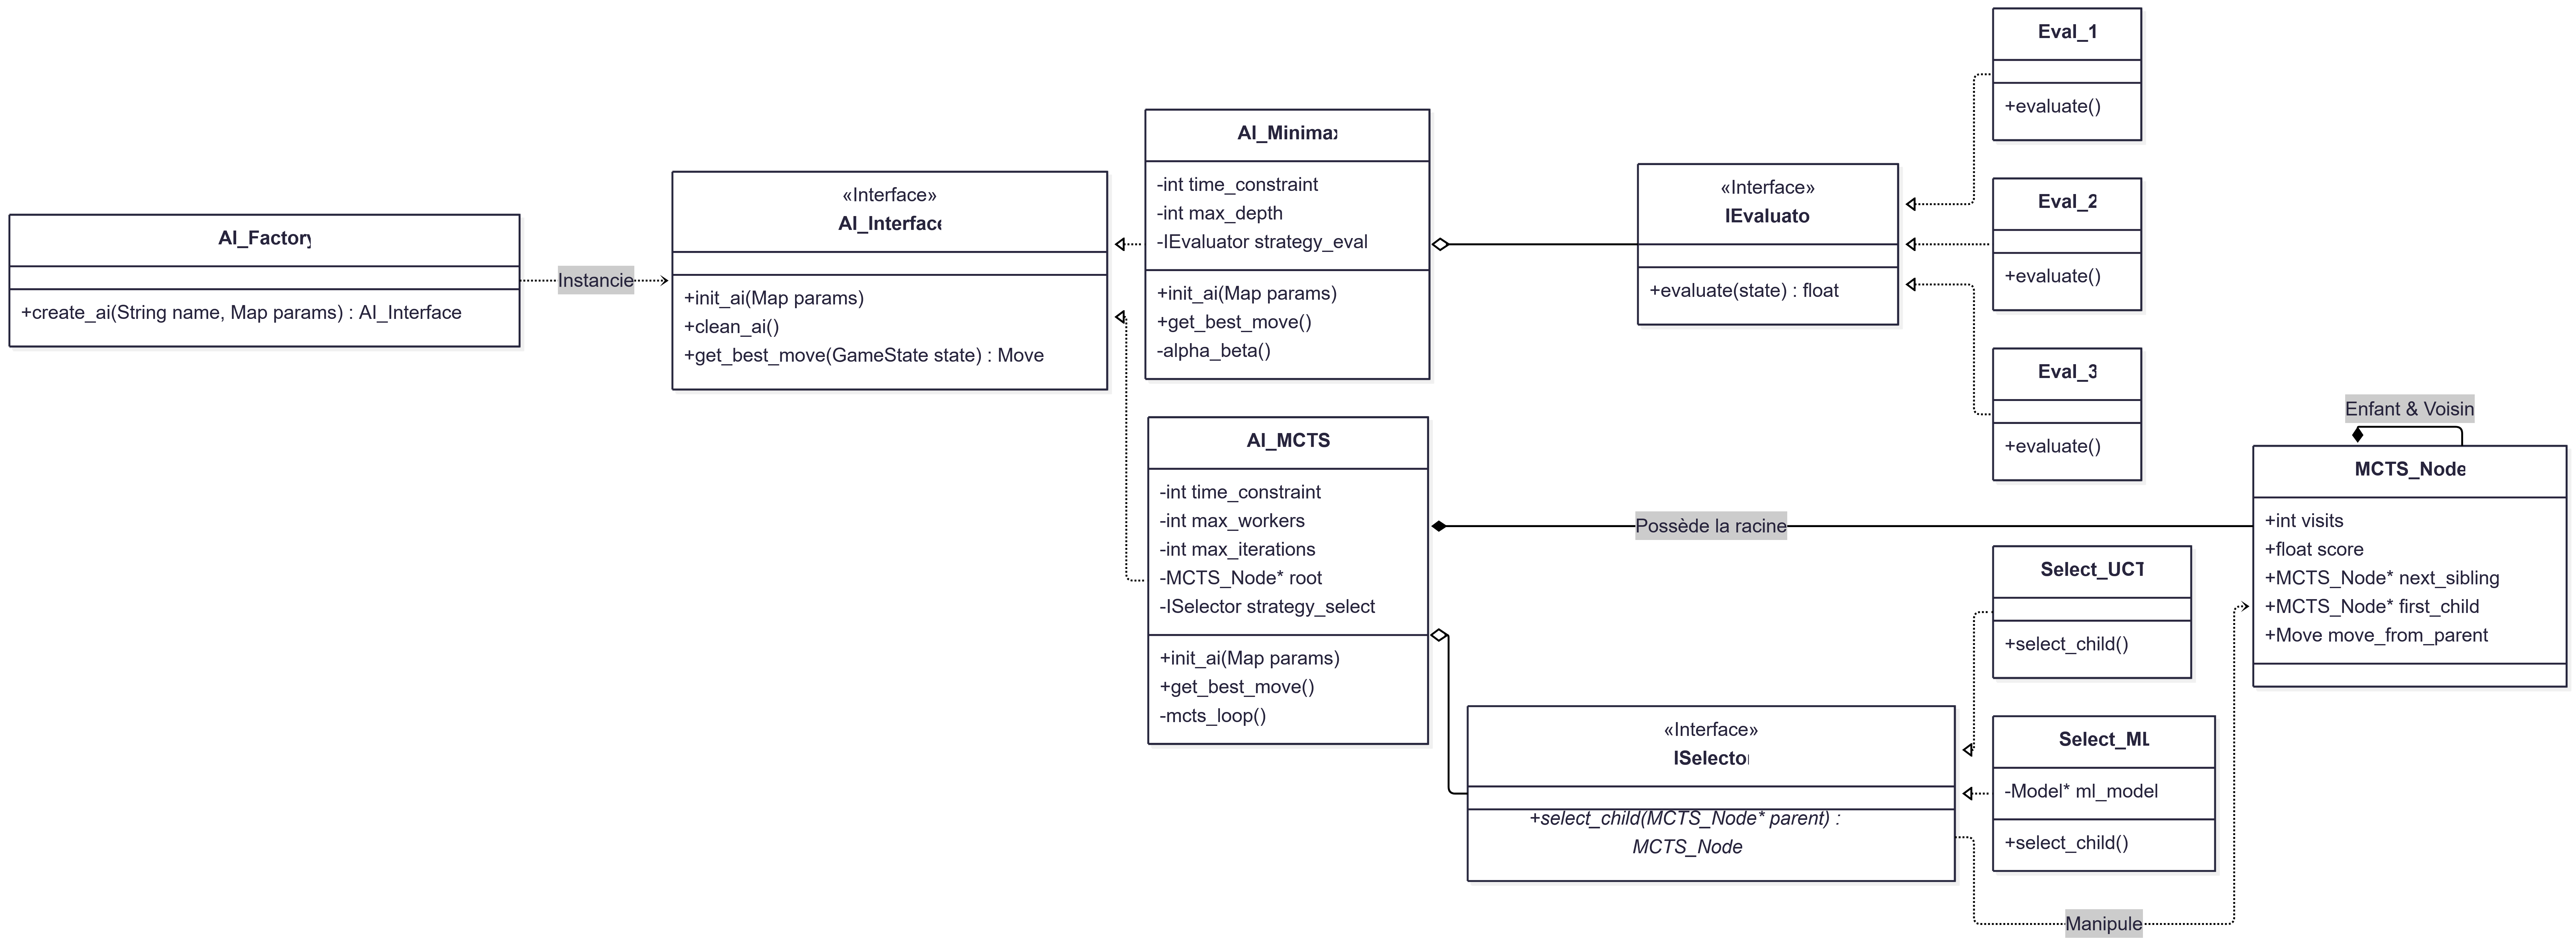
\includegraphics[width=0.85\paperwidth]{ia_uml.png}}
        \caption{IA - Diagramme UML}
        \label{fig:iauml}
    \end{figure}
    
    L'ensemble des éléments présents dans la Figure \ref{fig:iauml} seront donc présents au sein du module "IA", qui sera appelé pour le mode solo du jeu. Les paramètres donnés aux IA seront fournis directement par le GameEngine, qui les passera au sein d'un dictionnaire (map) lors de l'initialisation du mode de jeu seul, en fonction des paramètres définis par l'utilisateur (notamment max\textunderscore depth, time\textunderscore constraint, ...). La fonction d'évaluation (pour Minimax) et la fonction de sélection (pour MCTS) feront également partie de ces paramètres, et seront assignées via init\textunderscore ai.

    Comme précédemment cité \ref{sec:iastruc}, nous avons implémenté une structure d'arbre LCRS pour MCTS, et avons utilisé des interfaces pour le polymorphisme du code.

    La dépendance entre le module IA et les autres modules ne se fera que sur le module de jeu principal, où GameEngine utilisera AI\textunderscore Factory et gardera une référence à AI\textunderscore Interface afin d'utiliser la méthode "get\textunderscore best\textunderscore move"
    


    
    \section{Dépendances}
    \subsection{Réseaux}
    Pour ce qui est des dépendances de cette partie, on utilise essentiellement la bibliothèque native / système (POSIX) avec la Berkeley Sockets API, et  la librairie readline comme demandée dans le sujet.
    \section{Interfaces principales}

    
    \newpage
    \part{Spécifications} 
    \section{Réseaux}
    \subsection{Découverte de service}
    F38. Le client doit pouvoir voir automatiquement les serveurs de jeu actifs sur le réseau local via un broadcast, éliminant le besoin de connaître l'adresse IP cible à l'avance.

    Prérequis: Support du protocole UDP et configuration du socket avec l'option "SO BROADCAST".
      
    Architecture découplée : Le serveur utilise une structure (DiscoveryContext) pour émettre périodiquement des paquets (contenant : Nom du serveur, Port TCP, Statut) sans bloquer le jeu. Le client écoute sur un port  (ex: 8081). 
    
    Signatures des fonctions :
    
    Serveur : \begin{verbatim}void broadcast_presence(int udp_socket, int tcp_port,\end{verbatim} \smallskip \begin{verbatim} const char* server_name);\end{verbatim}
    
    Client : \begin{verbatim}server_list_t* client_scan_for_servers(int timeout_ms);\end{verbatim}
    
    Validation : Lancer une instance serveur sur une machine A. Sur une machine B (sans configurer préalablement), lancer la commande server list et vérifier que l'IP et le nom de la machine A apparaissent immédiatement. Vérifier avec Wireshark que les paquets UDP sont bien envoyés à l'adresse de diffusion 255.255.255.255.
    
    \subsection{Architecture Multi-clients et Routage} 
    F39. Le serveur doit avoir et garder plusieurs connexions TCP simultanées dans un seul processus et router les messages exclusivement entre les adversaires d'une même partie.
    
    Prérequis : Utilisation de l'appel système poll() pour le multiplexage d'entrées/sorties.
    
    Logique de routage : Associer chaque "socket fd" à un "game id" unique dans la structure ConnectedClient. Lors d'un SendMove, le serveur effectue une recherche pour trouver le socket pair en validant la condition : \begin{verbatim}(client.game_id == sender.game_id && client.fd != sender.fd)\end{verbatim}.

    \newpage
    Signature de la fonction : \begin{verbatim}void route_packet_to_opponent(server_context_t *ctx, packet_t *pkt,\end{verbatim} \smallskip \begin{verbatim} int sender_fd);\end{verbatim}
    
    Validation : Connecter 3 clients (Alice, Bob, Charlie). Alice et Bob lancent une partie (ID 1). Charlie attend en lobby (ID 0). Alice envoie un message. Vérifier que Bob reçoit le message, mais que le socket de Charlie ne reçoit aucune donnée.
    
    \subsection{Fiabilité du Flux et Reconstruction} 
    F40. Le système doit gérer la nature "flux" du protocole TCP en reconstruisant les messages applicatifs complets, indépendamment de la fragmentation réseau (paquets coupés ou collés).
    
    Prérequis : Allocation d'un buffer de réception persistant "tcp buffer" pour chaque client connecté et définition d'une constante "MAX BUFFER SIZE" pour éviter les débordements.
    
    Algorithme de reconstruction : À chaque recv(), les données sont ajoutées au buffer. Une boucle de parsing cherche le délimiteur de fin de commande (ex: \begin{verbatim}\n\end{verbatim} ou header de taille). Si une commande complète est trouvée, elle est extraite et traitée ; la mémoire restante est décalée au début du buffer via memmove.
    
    Signature de la fonction : \begin{verbatim}int process_incoming_stream(connected_client_t *client,\end{verbatim} \smallskip \begin{verbatim} network_events_t *callbacks);\end{verbatim}
    
    Validation : Test de robustesse : Créer un client "tricheur" qui envoie une commande de jeu octet par octet avec 10ms de pause entre chaque envoi. Vérifier que le serveur ne déclenche l'événement OnMoveReceived qu'une seule fois, au moment précis où le dernier octet est reçu, et que les données restent intègres.
    
    \part{Transparence IA}

    % --- Bibliographie ---
    \newpage
    \markboth{}{} 
    
    % 1. On l'ajoute au sommaire en tant que "part"
    \addcontentsline{toc}{part}{Références bibliographiques} 
    
    % 2. On crée le titre de la page (centré et gras comme une partie)
    \begin{flushleft}
        \huge\bfseries Références bibliographiques
    \end{flushleft}
    \vspace{1.5cm} % Espace entre le titre et la liste

    % 3. On affiche la liste
    \nocite{*} 
    \printbibliography[heading=none]

    \appendix



\end{document}